\documentclass[10pt, singlespace]{harvard-thesis}
\usepackage{epsfig,amsmath,amsthm,amssymb,multirow,color,xspace,fancyvrb,verbatim,url,listings,verbatim,alltt}
\usepackage{array, tabularx}
\usepackage{appendix}
\captionsetup{width=0.8\textwidth}

\usepackage{float}

\special{papersize=8.5in,11in}
\setlength{\pdfpagewidth}{8.5in}
\setlength{\pdfpageheight}{11in}

\usepackage{enumerate}
\newtheorem{theorem}{Theorem}[section]
\newtheorem{corollary}{Corollary}[theorem]

\theoremstyle{definition}
\newtheorem*{defn}{Definition}

\theoremstyle{remark}
\newtheorem*{eg}{Example}

\lstset{
       basicstyle=\ttfamily\small,
       keywordstyle=\color{blue}\ttfamily,
       stringstyle=\color{red}\ttfamily,
       commentstyle=\color{green}\ttfamily,
       morecomment=[l][\color{red}]{\/\/},
       morekeywords={true, false},
}

\graphicspath{{./figures/}}

\newcounter{notecounter}
\newcommand{\mynote}[1]{\stepcounter{notecounter}\textcolor{red}{\small \bf [\arabic{notecounter}]}\marginpar{\tiny \sf \textcolor{red}{\bf [\arabic{notecounter}]}#1}}

\newcommand{\lyt}[1]{\mynote{LYT: #1}}

\begin{document}

% some details about the thesis
\title{Concurrent Algorithms in Transactional Data Structures}
\author{Lillian Tsai}
\advisor{Professor Eddie Kohler}

% about the degree
\degree{Bachelor of Arts}
\field{Computer Science}
\degreeyear{2017}
\degreemonth{May}

% about the university
\department{Department of Computer Science}
\university{Harvard University}
\universitycity{Cambridge}
\universitystate{Massachusetts}

\maketitle
\copyrightpage
\abstractpage

\tableofcontents
\listoffigures
\listoftables

\dedicationpage
\acknowledgments

%\onehalfspacing
\singlespacing

\chapter{Introduction}
\section{STM and STO}
Parallelism is increasingly critical for performance in computer software systems, but parallel programming remains enormously challenging to get right. Low-level mechanisms for coordinating threads, such as lock-based strategies, are fragile and error-prone. To address this problem, researchers have developed programming tools and methodologies for managing parallelism. Prominent among these is software transactional memory (STM), which allows programmers to write concurrent code using sequential programming paradigms. By using STM, programmers reason about concurrent operations on shared memory through \emph{transactions}---atomic groups of operations---instead of single operations. 

Unfortunately, STM often results in high overhead and is rarely considered practical. To provide transactional guarantees, an STM system tracks the different memory words accessed within a transaction, and ensures that these words are not touched by concurrently executing transactions. Traditional word-based STM tracks all words of memory read or written in a transaction, incurring enormous overhead~\cite{cascaval}. To address this problem, a research team at Harvard has produced a novel type of STM, STO (Software Transactional Objects), that greatly improves upon the performance of traditional STM~\cite{sto}. The system's implementation works at a higher level than most previously developed systems: data structure operations, rather than individual memory words. For example, a word-STM tracks every word accessed in the path from the root during a binary search tree lookup, which introduces significant overhead from transactional bookkeeping and unnecessary conflicts: the transaction will abort if there is a concurrent update to the path, even though the result of the lookup may be unaffected. STO allows datatypes to track datatype-specific \emph{abstract objects} instead of memory words. Thus, during a binary search tree lookup, STO will track only the abstract object corresponding to the parent of the searched-for node, and use only this object to detect a conflict in which the node is modified, removed, or inserted. Compared to a word-STM, STO reduces the number of false conflicts and tracks hundreds of times fewer objects.

\section{Motivation}
The focus of this work is to make STO as fast as the fastest non-transactional, concurrent programming patterns available, and, when this is impossible, to characterize precisely why. Although STO outperforms traditional STM, STO’s performance still falls far below that of other concurrent programming paradigms, such as flat combining~\cite{flatcombining}. STO’s library of transactional datatypes---datatypes exposing transactional operations---allows programmers to add transactional memory to their programs. Thus, STO programs are only as fast as STO datatypes. Transactional data structure algorithms are therefore a natural focus for our research: by defining the limits and potentials of these algorithms, we learn how to maximize the performance of the STO system.

\section{Overview}
While the scope of our research includes all the different datatypes supported by STO, this thesis focuses on a few core data structures: queues and hashmaps. We began our research by implementing the initial version of these STO datatypes and, more broadly, developing design techniques for transactional data structures. These techniques define general patterns for designing transactional algorithms, such as how to handle reads and writes of the same object within the same transaction. These patterns, however, do not maximize scalability or performance.

To discover how to maximize performance, we analyze and compare the performance of existing STO data structures against implementations of highly-concurrent data structure algorithms from recent research. These concurrent data structure algorithms strive to maximize scalability and performance in a non-transactional setting: they ensure that single operations can execute concurrently in multiple threads, but provide no guarantees that a thread can execute a sequence of operations (a transaction) without interruption from another thread (atomically).
Transactional systems have strictly more work to do than these non-transactional concurrent systems: both systems must ensure correct synchronization of single operations, but a transactional system must also correctly synchronize multiple operations within a transaction such that they have atomic effect.
Thus, the performance of the fastest concurrent datatypes available acts as an upper bound for the performance that transactional STO data structures may reasonably hope to achieve. Our benchmarks highlight which concurrent, non-transactional data structures are the highest-performing, and which parts of the transactional data structure algorithms are bottlenecks and areas for improvement. 

We first hypothesize that combining concurrent, non-transactional programming patterns with our transactional design patterns will produce transactional datatypes that greatly outperform our previous implementations. To evaluate this hypothesis, we take the fastest concurrent datatype algorithms and implement them within the STO framework. We discover that the algorithmic changes necessary to move certain highly-concurrent data structures into STO results in a significant decrease in their performance; at times, they even underperform our initial STO data structures that use naive algorithms for concurrency.
Furthermore, our experience combining highly-concurrent, non-transactional algorithms with transactional algorithms leads us to conclude that reasoning about scalability in transactional datatypes is inherently different than reasoning about scalability in non-transactional, concurrent datatypes. In particular, to handle transactions, one must reason about invariants regarding the datatype's state during the entirety of the transaction's execution. We formalize this argument as a commutativity argument, drawing on previous work regarding commutativity in concurrent interfaces~\cite{scrule} and transactional objects~\cite{schwarz, weihl}.

The stateful nature of transactions, and therefore the reduced operation commutativity in a transactional setting, leads us to revise our hypothesis. 
We claim that certain highly-concurrent datatype algorithms may be intrinsically non-transactional, because the optimizations taken by these algorithms to achieve their high performance are incompatible with providing transactional guarantees. 
In other words, if the synchronization technique of a concurrent data structure relies on operation commutativity invalidated by transactional guarantees, then the data structure is unlikely to perform well in a transactional setting. 
If, however, there are few or no added commutativity constraints in a transactional setting, then the added synchronization costs to support transactions do not cripple the concurrent algorithm.
%Conversely, if transactional support can be added without modifying the synchronization algorithm, then we may retain the scalability and performance benefits of the concurrent data structure's algorithmic optimizations in a transactional setting.

To evaluate our claim, we take highly-concurrent data structures that underperform when integrated with STO, and investigate how these data structures act when we modify their \emph{specifications}---their operation interfaces---to allow for greater commutativity in a transactional setting. With an alternative specification, we achieve a better separation between the logic needed for transactional support, and the logic of the concurrent synchronization algorithm: this allows us to adapt concurrent data structures for transactional settings while retaining their high performance.
Comparing data structure performance in the original specification to performance in the alternative specification demonstrates the trade-off between the guarantees certain STO datatypes can provide, and their performance. For example, by preventing a thread from viewing the result of its read until its transaction completes, performance of the datatype more than doubles.

\subsection{Roadmap}
This work is divided into the following parts: 
\begin{itemize}
    \item Background information on transactions and transactional memory, and related work on transactional data structure algorithms and their scalability (Chapter~\ref{related_work})
    \item An evaluation of different transactional and concurrent algorithms for queue and hashmap data structures (Chapters~\ref{queue} and~\ref{hashmap})
    \item An explanation based on operation commutativity and invalid histories for why concurrent algorithms for queues fail to retain their performance and scalability in a transactional setting (Chapter~\ref{queue})
    \item A demonstration of how the performance loss of queue concurrent algorithms can be avoided through changing the queue operation specification to allow for greater commutativity in a transactional setting (Chapter~\ref{commutativity})
    \item A demonstration of, and explanation why highly-concurrent hashmap algorithms do retain performance and scalability in a transactional setting (Chapter~\ref{hashmap})
\end{itemize}


\chapter{Background and Related Work}
\label{related_work}

\section{Transactional Memory}
A transaction, or a group of operations that together form one logical unit of work, allows a programmer to more simply reason about concurrent access to shared state. The concept developed first in database theory, trickled into file systems, and expanded to other domains with the development of hardware transactional memory (HTM) in 1986 and software transactional memory (STM) in 1995~\cite{harristm}. 
A transaction is commonly defined by the ACID properties: atomicity, consistency, isolation, and durability. Transactional memory (TM)~\cite{harristm, herlihytm} guarantees transactional properties in shared memory; this differs from transactions in a database which (traditionally) work with data on disk.
TM is therefore unconcerned with the durability property: memory does not persist on some permanent medium. However, TM must still adhere to the remaining three ACI properties:

\emph{Atomicity} ensures that if a transaction commits, all changes made by the transaction are instantly visible to other actors performing transactions (for example, threads modifying shared memory or processes modifying a database); if a transaction aborts, none of the changes made by the transaction are visible to any other actor. Either all or none of the operations of the transaction should appear to succeed.

\emph{Consistency} guarantees that a transaction begins and ends with the state of the database or data structure satisfying particular (data structure-specific) invariants: for example, an invariant could be that the data structure is left in a state without duplicate entries.

\emph{Isolation} ensures that a transaction's execution appears to be isolated from any other transaction's (possibly simultaneous) execution. This allows for transactions to be \emph{serializable}, which means that one can find an ordering of committed transactions that satisfies the observed history of results. In this ordering, it should appear as if operations within one transaction are never interleaved with operations in another transaction. 

Transactional memory transactions also are \emph{linearizable}~\cite{linearizability}: all transactions performed at a later clock time than a committed transaction observe the changes made by the committed transaction. This allows programmers to easily determine the order and effects of transactions.


Systems implementing transactional memory can be optimistic, pessimistic, or some combination of the two, and may use eager and/or lazy updates~\cite{harristm}. 
Optimistic transactional memory systems and pessimistic transactional memory systems both track the transaction's intended changes in the transaction's \emph{write set} and any state observed during the transaction in the transaction's \emph{read set}. 
An optimistic system checks for invalidated values in the read set only at commit time. If all values are valid, the system performs the changes in the transaction's write set and the transaction is marked committed. Otherwise, the transaction aborts and the system ensures that the transaction leaves no visible effects (potentially rolling back any changes the transaction has made). An optimistic system therefore assumes (optimistically) that no other thread will conflict with another thread's transaction, and executes all operations of the transaction before it checks if any conflict has indeed occurred.

A pessimistic transactional system instruments every read and write with additional checks to see if another thread is simultaneously accessing the same part of memory and creating a conflict. If any such conflicts are detected during the read or write, then the thread either aborts or stalls until the conflicting transaction completes by either committing or aborting. A pessimistic approach therefore assumes that multiple threads will often be modifying or reading memory at the same locations during their transactions' executions. 

Transactional memory systems also practice eager updates or lazy updates. A system is eager when it updates shared memory during the transaction's execution. It maintains an ``undo'' log of changes, which is used if the transaction aborts and the changes need to be undone. 
A system is lazy when no changes are done until the transaction commits: all intended changes during execution are buffered by the system or written to a log and applied at commit time. Systems can range from fully eager to fully lazy, with most practicing a mix of the two techniques.

Transactional systems can also provide the \emph{opacity} property~\cite{opacity}, a property that guarantees that the code running transactions will never observe an inconsistent memory state. 
In other words, all the transaction's reads must be consistent with a single snapshot of memory at some point during the transaction.
Opacity is necessary to avoid potential failures such as infinite loops and invalid pointer dereferences. With opacity, a transaction will abort immediately upon observing an inconsistent state that would cause the transaction to fail at commit time. Note that pessimism does not guarantee opacity: a transaction performing read-only operations will not acquire locks on the data structure, and may therefore observe an inconsistent state at some point during its execution.
In certain systems such as STO, providing opacity requires keeping track of a global transaction ID (TID). This global TID is used to check the consistency of previously read items when the transaction observes a memory state. The TID is updated whenever a transaction commits and modifies memory. Opacity hinders the performance of the code running transactions because this TID must be accessed whenever a transaction accesses memory (to check the state of previously read items) and when a transaction commits. In our benchmarks, we disable opacity---allowing for the possibility of rare failures caused by memory inconsistencies---for the sake of performance. We benchmark transactional data structures without opacity enabled to measure our transactional system at its maximum achievable performance.

\section{Transactional Memory Systems}
Transactional Memory can be implemented in both hardware and software. Although hardware transactional memory (HTM) naturally outperforms software transactional memory (STM), a purely hardware TM has several inherent limitations. HTM will fail when the working sets of the transactions exceed hardware capacities; for example, the buffer used to track read and writes of the transaction is restricted in size. In addition, HTM lacks flexibility (granularity of reads/writes is at the word level) and fails to be truly composable~\cite{htm}. Nevertheless, with the increasing support for HTM in computer hardware~\cite{intel_htm}, integrating STM with HTM offers performance improvements over what STM alone can achieve.

The STO system~\cite{sto} used by this work is one of several STM systems. For simplicity, we can generalize STMs into three groups: word/object-based STMs, which track individual memory words or objects touched during a transaction, STMs that expose non-transactional API for performance gains, and abstraction-based STMs which track items based on abstract datatypes.

TL2~\cite{tl2} and LarkTM~\cite{larktm} are highly-optimized word-STMs that track memory words touched during a transaction. SwissTM~\cite{swisstm} is also a word-STM, but increases performance by tracking memory in 4-word groups, resulting in less overhead than tracking individual memory words. There have also been object-based STMs which track objects instead of memory words, but incur extra cost by shadow copying any objects written to within the transaction~\cite{stm_objects}. 

Open nesting~\cite{opennesting}, elastic transactions~\cite{elastic}, transactional collection classes~\cite{tcc}, early release~\cite{earlyrelease}, and SpecTM~\cite{spectm} are techniques for implementing transactions that, like STO, speed up transactional performance by reducing the bookkeeping costs and the number of false conflicts. However, these techniques expose non-transactional APIs to the programmer, which requires the programmer to be an expert in the system in order to implement transactions. This complicates, rather than simplifies, concurrent programming. For example, transactional collection classes remove unnecessary memory conflicts in data structures by wrapping the datatype with semantic locks; this requires designing multi-level, open-nested transactions, and presents a much more complicated framework than does STO, which allows the datatype to be designed specifically to support transactions.

STO is one of several STM systems that use abstraction to improve STM performance~\cite{predication,autolock, optboost, boost}. These systems expose a transactional API to programmers in the form of concurrent, transactional data structures that are written on top of an STM. However, systems other than STO build their data structures on top of traditional word-STMs, whereas STO builds data structures on top of an abstract STM which tracks abstract items defined by each data structure. This lets STO improve performance beyond that of previous systems. 

Our work focuses on datatypes and how they perform within transactional settings. We now take a closer look at STO and other abstract STM systems that expose an API in the form of transactional data structures allowing programmers to use transactions.

\section{Abstraction-based STMs}

The STO system tracks the abstract operations of a transactional abstract datatype. STO consists of a core system that implements a transactional, optimistic commit-time protocol, and an extensible library of transactional datatypes built on top of this core. While programmers can use the many transactional datatypes already implemented in STO (ranging from queues to red-black trees), STO provides a transactional framework that allows programmers to easily add transactional support to other datatypes based on their particular semantics. STO allows datatypes to add datatype-specific \emph{items} to their read or write sets, thereby reducing bookkeeping costs by 
exploiting the semantics of the particular datatype. 

Many datatypes enforce transactional correctness using \emph{versions} that correspond to items. A version acts as a lock on the data structure: in order to update the data structure, a thread must first lock the version. A version tracks changes to the data structure by monotonically increasing whenever a thread modifies corresponding data structure item. Thus, any version seen by a thread is equivalent to some previous or current state of the data structure. When a transactional operation performs a read of some data structure state, it adds a read of the corresponding version value. This read version value is checked when the transaction commits to ensure that the observed data structure state is still valid: if the version value has changed, then the data structure state has changed as well.
The version's value from the \emph{first} time we perform a read of the version is validated at commit time; this ensures that every observed state since the start of the transaction is still valid.

STO also allows datatypes to use a variety of different concurrency control algorithms. For example, STO's transactional hashmap defines abstract items for each bucket, which are invalidated only when the bucket size changes. This means that transactions conflict only when modifying or reading the same bucket, allowing scalable access to the data structure. In addition, at most one item is added to the read- or write-set per operation, which can be orders of magnitude fewer than the number of items tracked by a word- or object-based STM. STO allows datatypes to define their own strategies for transaction execution: a datatype can insert elements during transaction execution (eagerly) or wait until commit time to insert (lazily). The specifics of the commit protocol are implemented as datatype callbacks. This allows a datatype to use pessimistic strategies for certain operations (e.g., by needing to acquire a lock) while using optimistic strategies for other operations. STO is therefore a flexible hybrid of optimistic/pessimistic and eager/lazy versioning strategies.

Boosting~\cite{boost} is a method to convert highly-concurrent (non-transactional) data structures into transactional data structures. Like STO, boosting determines conflicts between transactions by relying on a particular data structure's semantics. Instead of allowing each datatype to define read- and write-set items, however, boosting maps a datatype's operations to abstract locks. If two operations do not commute---i.e., swapping the order of their invocations affects the final state of the data structure or the responses returned by the operations---then the abstract locks for the operations will conflict: for one of the operations to be performed, both the abstract lock for that operation and the abstract lock for the conflicting operation must be acquired.
Thus, the granularity of synchronization of the original linearizable data structure is only achievable for commutative operations in its boosted form. Because a transaction may abort, boosting practices undo logging and requires that each operation has an inverse. These constraints prevent boosting from applying to all data structures, but make it particularly useful for ones like sets. Unlike boosting, STO allows us to work with data structures whose operations have no inverse. Boosting is an inherently pessimistic strategy, using eager versioning, whereas STO allows for a hybrid approach that can improve performance.

Optimistic boosting~\cite{optboost} is a technique meant to improve the performance of boosting. It proposes an optimistic approach in which acquisition of the abstract locks is delayed until commit time. During execution, semantic items are added to the read- and write-sets of the transaction and validated at commit time; if all reads are valid, then the appropriate abstract locks are acquired and modifications applied to the data structure. Because execution is optimistic and abstract locks are not eagerly acquired at the higher, ``boosted'' level, the underlying concurrent data structure can be lazy and wait until commit time to execute operations. This adds support for operations that may not have an inverse. 
However, optimistic boosting has not been shown to be effective in practice. STO provides a more flexible hybrid transactional framework and achieves larger performance gains than has been demonstrated by optimistic boosting.

Automated locking~\cite{autolock} takes a similar approach to boosting by pessimistically acquiring abstract locks corresponding to each operation. It differs from boosting because it also takes a datatype-specific commutativity specification of conditions in which operations commute. The commutativity specification of an abstract datatype is compiled into a symbolic set (called a ``locking mode'') that is used to prevent conflicting operations from being run concurrently. If two operations commute, the ``locking mode'' allows them to run concurrently.
This approach optimizes and automates the creation of abstract locks for an abstract data structure. A similar approach may help STO data structures choose which abstract read and write items to track during a transaction to avoid false conflicts.

Predication~\cite{predication} is a technique that maps operations to ``predicate words'' contained in a shared-memory table managed by the STM. Each predicate word represents a property of the data structure. For example, looking up an element $e$ in a set would be associated with an \texttt{\{in\_set?($e$)\}} predicate word, and the STM would add reads or writes of the predicate word when $e$ is removed or added to the set. 
Unlike boosting, transactional predication achieves semantic conflict detection without keeping an undo log. However, predication must insert predicate words into the table for absent as well as present lookups, causing a garbage collecting problem that STO and other systems do not face. Transactional predication also focuses on making transactional data structures perform equally as well as highly-concurrent data structures in non-transactional settings. This is orthogonal to our work here and can be a future line of optimization for STO data structures.

The Transactional Data Structures Libraries (TDSL)~\cite{tdsl}, like STO, produces collections of transactional data structures for programmers to use. Similar to STO, TDSL allows for both pessimistic and optimistic, and eager and lazy strategies and customizes strategies for each individual data structure. This allows for optimizations that rely on the data structure's semantics. Unlike STO, data structures in TDSL are also optimized for single-operation transactions (which we see as an orthogonal line of work). While TDSL contains only a queue and skiplist, STO has implementations of many other data structures in transactional settings, including a queue, hashmap, list, priority queue, and red-black tree. Our work in this thesis draws upon some of the algorithm designs for the queue implemented in TDSL.

This thesis investigates the integration of several highly-concurrent (non-transactional) data structures with STO. In particular, we test and modify different concurrent queue and concurrent hashmap algorithms, which we describe in more detail in Chapters~\ref{queue} and~\ref{hashmap}. Similar work has been done with lazy sets~\cite{lazyset}, in which transactional support is added to a lazy concurrent set. We extend their work to other data structures and investigate further how to achieve performance close to highly concurrent, non-transactional data structures.

\subsection{Commutativity in Transactional Data Structures}

STO, along with the above methods of integrating concurrent abstract datatypes with STM, builds upon the ideas introduced by Weihl in the late 1980s~\cite{weihl}. Weihl defines optimal local atomicity properties of datatypes that allow for transactions to be serialized, therefore providing an upper bound on the amount of concurrency achievable in transactional datatypes. These local properties are derived from algebraic properties of the data structure, such as commutativity of particular operations. Weihl also demonstrates an inherent relation between commutativity-based concurrency control and transactional recovery algorithms. Unlike our work with STO, however, Weihl does not focus on the implementation of these properties.

Schwarz and Spector~\cite{schwarz} introduce a theory for ordering concurrent transactions based on the semantics of shared abstract datatypes and dependencies of different datatype operations. For each operation, the programmer specifies the operation's preconditions, postconditions, and invariants. To describe interactions between operations in a transaction, the programmer additionally provides an interleaving specification. This defines dependency relations between datatype operations. From this set of dependency relations, Schwarz and Spector can define the limits of concurrency for the datatype by drawing upon results from Korth~\cite{korth} which show that when two operations commute (have no inter-dependencies), the order in which the operations are ordered do not affect serializability. We discuss this work further in Chapter \ref{commutativity}. 

Schwarz and Spector also demonstrate that increased concurrency can be achieved by weakening the serializability of transactions: once the semantics of a datatype have been taken into account, the remaining constraints on concurrency come from enforcing transactional properties~\cite{kung}. Weaker ordering properties allow a datatype to fully exploit its operations' semantics. They exemplify this with a WQueue design: a higher-concurrency queue with modified semantics that preserves a weaker ordering property than serializability. However, their paper focuses on the theoretical result instead of the implementation and is not concerned with explicit concurrent algorithms for the queue. Our work in Chapter \ref{commutativity} with the weakly-transactional queue builds off this idea of a weaker transactional specification, and we provide experimental evidence that operation semantics can be usefully exploited only by providing weaker transactional guarantees.

Badrinath and Ramamritham~\cite{badrinath} investigate operation commutativity to define recoverability, a weaker notion of commutativity that can achieve enhanced concurrency. Their key observation is that recoverability, unlike commutativity, takes into account the \emph{removal} of operations from the execution history. If an operation is recoverable with respect to another transaction's operation, then the operation can be eagerly applied to the data structure without the other transaction's operation aborting or committing. Although this technique forces an ordering at commit time, it has the nice property that at least one of the transactions will be able to commit. This prevents issues such as cascading aborts, in which one transaction's abort causes the abort of another transaction, which can cause the abort of a third transaction (and so on).
Commutativity has also played a role in network consistency algorithms and conflict-free replicated data types (CDRTs)~\cite{CRDT}, as well as in the database community.

Kulkarni, et.al.~\cite{galois} define the notion of a commutativity lattice (predicates between pairs of methods) to reason about commutativity in a data structure. The Galois system, upon which this idea is tested, provides a framework in which the programmer defines a commutativity lattice for individual data structures and, by exploiting commutativity, improves the performance of irregular parallel applications. Galois, however, focuses on constructing commutativity checkers instead of serializing transactions.

Finally, commutativity work has played a large part in optimizing distributed transactions. Mu, et.al.~\cite{distributed} introduce a system, ROCOCO, that first distributes pieces of concurrent transactions across multiple servers. These servers then determine dependencies between their pieces of concurrent transactions and delay all transaction execution until commit time. When a transaction commits, its corresponding dependency information is sent to all servers via a coordinator, allowing the servers to re-order conflicting pieces of the transaction and execute them in a serializable order. This reduces aborts and unnecessary conflicts.


\chapter{FIFO Queue Algorithms and Analysis}
\label{Queue}

This chapter investigates different concurrent and transactional algorithms for queues to draw conclusions about concurrent queue algorithms in transactional settings. We begin with an overview of concurrent and transactional queue specifications and algorithms. We then evaluate how these queues perform on several microbenchmarks. Given our results, we conjecture that highly-concurrent queue algorithms are inherently unsuited to be converted for use as a fully transactional queue algorithm.

\section{Transactional Queue Specification}

A concurrent queue must adhere to the following specification, in which all operations can be ordered such that:
\begin{itemize}
    \item A value is popped off the queue only once (no duplicate pops)
    \item A value is pushed onto the queue only once (no duplicate pushes)
    \item Values are popped in the order in which they are pushed
\end{itemize}

A transactional queue adds the following invariants to the specification; there must be a serial order of all transactions such that, within one transaction:
\begin{itemize}
    \item Any two pops pop consecutive values in the queue starting from the head of the queue 
    \item Any two pushes push consecutive values at the tail of the queue
\end{itemize}

To satisfy these invariants, transactional data structures must support \emph{read-my-writes}. This is when a thread sees and modifies or returns the value from a previous operation in the transaction.

%%%%%%%%%%%%%%%%%%%%%%%%%%%%%%%%%%%%%%%%%%%%%%%%%%%%%%%%%%%%%%%%%%%%%%%%%%%%%%%%%%%%%%%%%%%%%%%%%%
\section{STO Queue Algorithms}

STO provides a transactional FIFO queue that adheres to the interface exposed by the C++ standard library queue. Our first transactional algorithms were designed with transactional correctness in mind, and concurrency as a secondary concern. Here we detail different transactional queue algorithms that we implemented in this fashion.

The STO data type algorithms enforce transactonal correctness using \emph{versions}. A version can act as a lock on the data structure: in order to update the data structure, a thread must first lock the version. A version also tracks changes to the data structure because it monotonically increases when a thread modifies the data structure. Thus, any version seen by a thread is equivalent to some previous or current state of the data structure. The first instance of the version observed by a thread during a transaction is checked when the transaction commits. This ensures that all observations are valid. Note that we cannot update the read version to an instance of the version observed later in the transaction. This is because we need to validate the first time we see the version in the transaction. 

\subsection{STO1 Queue}
The STO1 Queue is the first implementation of the transactional queue data structure using STO's framework. It implements a circular, fixed-size transactional queue.

The queue is implemented using optimistic concurrency control (OCC), which is a transactional algorithm that optimistically assumes that no other transaction will conflict with a thread's transaction. No thread prevents another thread from operating simultaneously on the queue during a transaction, which means multiple threads can add read/writes of the same parts of the queue during their transactions. Contention only occurs during commit time, when the thread must necessarily lock the queue so that it can safely verify and modify the queue's values without parallel modifications by other threads. A thread can only realize that another thread has “beaten” it to modifying the queue at commit time.

There are two versions for the queue that can potentially invalidate a transaction if either changes: a headversion, and a tailversion. The headversion tracks the location of the head of the queue, and the tailversion tracks the location of the tail of the queue.

The queue supports three transactional operations: push, pop, and \texttt{front}. A push within a transaction adds to an internal \texttt{write\_list\_item}. This \texttt{write\_list} holds thread-local list of values to be pushed onto the queue, which are added to the tail of the queue during commit time (ensuring all values are added consecutively). We observe that all transactions comprised of only pushes will always commit because pushes do not observe any property of the queue: one transaction's pushes, \texttt{front}s, or pops do not affect the outcome of another's pushes. (Note, however, that the opposite is not true). During commit time, the thread locks the tailversion so that no other thread's push can push onto the queue. The items on the \texttt{write\_list} are added to the queue, and the tailversion incremented.

A pop within a transaction first checks if the queue is empty. If the queue is empty, then the thread reads the tailversion to ensure that no other transaction has committed a push before this thread commits. Suppose another thread successfully installs a push before this thread commits. Then this pop should have read that pushed value instead of seeing an empty queue. This forces the thread to abort the transaction. If there have been items added to the \texttt{write\_list} from previous pushes within the transaction, then the pop will “pop” an item off the \texttt{write\_list}, performing an instance of \emph{read-my-writes}. Such a modiicatio is allowable during execution time because the \texttt{write\_list} is thread-local. If the queue is nonempty, then the thread reads the headversion to ensure that no other transaction has committed a pop before this thread commits. The thread then finds the item to pop off the queue by iterating through the queue from the head until it finds an item that has not yet been popped off within this transaction. The thread adds a write to this item so it knows during commit time and during future pops that it intends to pop this item.

A \texttt{front} within a transaction is similar to a pop, excluding the iteration procedure to find the item to return (the value at the head of the queue or the \texttt{write\_list} is always returned). The queue is not modified, but the versions are read appropriately to ensure that the values returned by the \texttt{front} are still valid at commit time.

The design is summarized in Table \ref{table:sto1}.

\subsection{STO2 Queue}
The STO2 Queue is also a circular, fixed-size queue, with operations push, pop, and \texttt{front}. The STO2 Queue algorithm is a hybrid design integrating the STO1 algorithm with another transactional algorithm: pessimistic locking. This takes inspiration from the transactional queue from the Transactional Data Structures Library [1] as described in previous work. Their pessimistic transactional queue appears to achieve better performance in their benchmarks than the STO1 queue, and the algorithm is simpler to implement and describe. 

Pessimistic locking entails locking the queue when any naturally-contentious operation---pop or \texttt{front}--- is invoked. The queue is then only unlocked after the transaction is complete. This ensures that no other thread will execute an operation that may invalidate a pop or \texttt{front} within this thread's transaction. However, operations such as ``push'' that can operate without any wait do not require locking during execution. Therefore, a push follows the same protocol as in the STO1 queue.

Because pop and \texttt{front} lock the queue, there are no conflicts at commit time. A thread only aborts if it fails to obtain the lock after a bounded period of time. The one version, “queueversion,” acts as the global queuelock. 

The design is summarized in Table \ref{table:sto2}

%%%%%%%%%%%%%%%%%%%%%%%%%%%%%%%%%%%%%%%%%%%%%%%%%%%%%%%%%%%%%%%%%%%%%%%%%%%%%%%%%%%%%%%%%%%%%%%%%%

\section{Flat Combining Queue Algorithms}
Given the relatively slow performance of our STO queues, we looked to find a highly-concurrent (non-transactional) queue algorithm that would be promising to integrate with STO's transactional framework. After running several benchmarks (see Figure \ref{fig:concurrent_queues}), we found the most promising to be the Flat-Combining technique, which not only outperforms other queue algorithms, but also addresses several of the bottlenecks we observe in the STO queues.

\subsection{Flat Combining Queue (Non-Transactional)}
\label{fcqueuent}

\emph{In the following discussion of our flat combining-based queues, we omit the discussion of the \texttt{front} operation to simplify reasoning about the state of the queue. An appropriate algorithm for \texttt{front} can be easily inferred from those used for pop.}

Flat Combining, proposed by Hendler, et. al. in 2010\cite{flatcombining}, is a synchronization technique that is based upon coarse-grained locking and single-thread access to the data structure. The key insight is that the cost of synchronization for certain classes of data structures often outweighs the benefits gained from parallelizing access to the data structure. These data structures include high-contention data structures such as stacks, queues, and priority queues. Created with this insight, the flat combining algorithm proposes a simple, thread-local synchronization technique that allows only one thread to ever access the data structure at once. This both reduces synchronization overhead on points of contention (such as the head of the queue) and achieves better cache performance by leveraging the single-threaded access patterns during data structure design.

The data structure design includes a sequential implementation of the data structure, a global lock, and per-thread records that are linked together in a global publication list. A record allows a thread to publish to other threads the specifics of any operation it wants to perform; the result of the operation is subsequently written to and retrieved from the record.

When a thread T wishes to do an operation O:
\begin{enumerate}
    \item T writes the opcode and parameters for O to its local record. Specifically for the queue, the thread writes \texttt{<PUSH, value>} or \texttt{<POP, 0>} to its local record.
   \item T tries to acquire the global lock.
   \begin{enumerate}
        \item T acquires the lock and is now the “combiner” thread. T applies all thread requests in the publication list to the data structure in sequence, and writes both the result and an \texttt{<OK>} response to each requesting thread's local record.
        \item T failed to acquire the lock. T spins on its record until another thread has written the result to T's record with the response \texttt{<OK>}.
    \end{enumerate}
\end{enumerate}

In the context of the queue, flat combining proves to be an effective technique to handle the contention caused by parallel access on the head and tail of the queue. In addition, their choice of queue implementation uses ``fat nodes'' (arrays of values, with new nodes allocated when the array fills up), which both improves cache performance and allows the queue to be dynamically sized. Both the STO1 and STO2 queues suffer from the contention and cache performance issues pointed out in the flat combining paper, leading us to believe that flat combining's alternative synchronization paradigm might improve the performance of a transactional queue as much as it does for a concurrent queue.

\subsection{Flat Combining Queue (Transactional)}

Recall that, in addition to the requirements for a correct concurrent queue, a transaction queue must guarantee that there must be a serial order of all transactions such that, within one transaction, any two pops pop consecutive values in the queue starting from the head of the queue and any two pushes push consecutive values at the tail of the queue.

In order to add transactional guarantees to the flat combining queue, the order in which threads' requests are applied to the queue becomes important. For example, let a transaction in thread T1 be \texttt{pop, pop} and a transaction in thread T2 be pop. The combiner thread sees \texttt{T1:pop} and \texttt{T2:pop}, and applies both operations to the queue. T1 second pop request will violate the transactional specification because the two popped values in T1's transaction will not be consecutive. T1 must now abort, which means T2's pop is now invalid: it does not represent a pop at the head of the queue.

Addressing the scenario described above requires two important changes to flat combining (we describe the rational for these changes in Chapter~\ref{commutativity}): 
\begin{enumerate}
\item pushes cannot be applied to the queue during a transaction's execution, and must instead be performed when a transaction commits
\item An uncommitted pop in a thread's transaction must be unobservable by any other thread. This can be implemented in two ways:  
    \begin{enumerate}
        \item The algorithm can delay a transaction's pops until commit time. This algorithm must track which values in the queue are going to be popped within the transaction. This prevents duplicate pops and detects if the queue will be ``empty'' given how values will be popped.
        \item The algorithm does not execute flat combining requests from other threads until the transaction has committed or aborted. This can be implemented either through making other threads' transactions abort, or by causing the threads to block or spin.
    \end{enumerate}
\end{enumerate}

We now describe the new algorithms for push and pop.  We change the types of request a thread can publish to its record on the publication list. Recall that the original flat combining queue supports two requests: \texttt{<PUSH, value>} and \texttt{<POP, 0>}. The transactional queue supports the follow requests:
\begin{itemize}
    \item \texttt{<PUSH, list>} : push a list of values onto the queue
    \item \texttt{<MARK\_POP, thread\_id>} : mark a value in the queue to be popped by this \texttt{thread\_id}
    \item \texttt{<DEQ, thread\_id>} : dequeue all values in the queue that are marked by this \texttt{thread\_id}
    \item \texttt{<EMPTY?, thread\_id>} : check if the queue, after popping all items marked by this \texttt{thread\_id}, is empty
    \item \texttt{<CLEANUP, thread\_id>} : unmark all values that are marked with this \texttt{thread\_id}
\end{itemize}

As with the STO1 queue, a push within a transaction adds to an internal \texttt{write\_list\_item}. At commit time, the thread will invoke the \texttt{<PUSH, list>}, with the \texttt{write\_list} passed as the argument.

A pop is implemented with a pessimistic approach. Performing a pop within a transaction invokes the \texttt{<MARK\_POP, thread\_id>} command. The combiner thread, upon seeing a MARK\_POP command, looks at the first value at the head of the queue. If this value is marked with another thread's \texttt{thread\_id}, the combiner thread returns \texttt{<ABORT>} to the calling thread.

If the value is not marked, the combiner thread marks the value with the caller's \texttt{thread\_id} and returns \texttt{<OK>}. Else the value is marked by the calling thread's \texttt{thread\_id}. Note that in this scenario, no other thread can have marked values in the queue, since they will abort when seeing the head value marked by the calling thread's \texttt{thread\_id}. The combiner thread iterates sequentially through the queue values until it reaches a value not marked by the calling thread's \texttt{thread\_id}. It then marks the value with the caller's \texttt{thread\_id} and returns \texttt{<OK>}. Upon receiving the response, the calling thread adds a write to a \texttt{pop\_item} to tell the thread to post a \texttt{<DEQ, thread\_id>} request at commit time. This removes the popped value from the queue.

If the queue is either empty or there are no values not marked with the caller's \texttt{thread\_id}, the combiner thread will return \texttt{<EMPTY>}, which is remembered by the calling thread. An \texttt{<EMPTY>} response requires that the size of the queue be checked at commit time.

Note that this algorithm does not allow pops to read the values pushed within the same transaction. To do so would require passing in the thread's \texttt{write\_list} in addition to the \texttt{thread\_id} as arguments to the combiner thread. During our evaluation, we leave this part of the transactional queue specification unimplemented (and expect that adding this will only decrease performance).

The \texttt{<EMPTY?, thread\_id>} request is posted when a thread attempts to commit a transaction that observed an empty queue at some point in its execution. This happens when the thread receives an \texttt{<EMPTY>} response to a \texttt{<MARK\_POP>} request during the transaction. If the response to \texttt{<EMPTY?>} is true, then the thread knows that no other thread has pushed onto the queue between the time of its \texttt{<MARK\_POP>} seeing an empty queue and commit time. Else another thread has pushed items onto the queue, invalidating this thread's pop result, and this thread must abort.

If a thread ever sees an empty queue when executing a pop \emph{and} subsequently performs a push within the same transaction, the thread must prevent another transaction from committing between the time of the empty check and the installation of its pushed value. This requires adding what is essentially a lock of the tail of the queue. This is implemented via additional machinery in the combiner thread, which signals whether or not a transaction has locked the queue, and prevents any other thread's pushes from being installed until the ``lock'' is released.\lyt{TODO ACTUALLY IMPLEMENT}

The \texttt{<CLEANUP, thread\_id>} request is posted when a thread aborts a transaction and must unmark any items in the queue that it had marked as pending pops. The combiner thread iterates through the queue from the head and unmarks any items with the \texttt{thread\_id}.

The algorithm is summarized in Table \ref{table:fcqueue}.

\begin{table}[ht!]
    \scriptsize
\centering
\begin{tabular}{|c|c|c|c|c|l|}
\hline
    \multicolumn{2}{|c|}{Operation} & Execution-Time Effects & Read Set & Write Set & \multicolumn{1}{c|}{Commit Protocol} \\ 
    \hline\hline
    \multicolumn{2}{|c|}{Push} & none & none & \texttt{write\_list}& 
        \begin{tabular}[c]{@{}l@{}}- lock tailversion\\ - perform pushes\\ - increment tailversion\\ - unlock tailversion\end{tabular}\\ 
    \hline
    \multirow{2}{*}{Pop} & Nonempty & none & headversion & element to be popped & \begin{tabular}[c]{@{}l@{}}- lock headversion\\ - check headversion\\ - perform pops\\ - increment headversion\\ - unlock headversion\end{tabular} \\
    \cline{2-6} 
                     & Empty & none & tailversion & none  & 
                     \begin{tabular}[c]{@{}l@{}}- lock tailversion\\ - check tailversion\\ - unlock tailversion\end{tabular} \\
\hline
\end{tabular}
\caption{The STO1 Queue Algorithm}
\label{table:sto1}
\end{table}

%%%%%%%%%%%%%%%%%%%%%%%%%%%%%%%%%%%%%%%%%%%%%%%%%%%%%%%%%%%%

\begin{table}[ht!]
    \scriptsize
\centering
    \begin{tabular}{|c|c|c|c|c|l|}
\hline
    \multicolumn{2}{|c|}{Operation} & Execution-Time Effects & Read Set & Write Set & \multicolumn{1}{c|}{Commit Protocol} \\ 
    \hline\hline
    \multicolumn{2}{|c|}{Push} & none & none & \texttt{write\_list}& 
        \begin{tabular}[c]{@{}l@{}}- lock queueversion,\\ - perform pushes,\\ - increment queueversion\\ - unlock queueversion\end{tabular}\\ 
    \hline
    \multirow{2}{*}{Pop} & Nonempty & lock queueversion & none & element to be popped  & \begin{tabular}[c]{@{}l@{}}- perform pops\\ - unlock queueversion\end{tabular} \\
    \cline{2-6} 
                     & Empty & lock queueversion & none & none & none\\
\hline
\end{tabular}
    \caption{The STO2 Queue Algorithm (delayed pop execution)}
\label{table:sto2}
\end{table}

%%%%%%%%%%%%%%%%%%%%%%%%%%%%%%%%%%%%%%%%%%%%%%%%%%%%%%%%%%%%
\begin{table}[ht!]
    \scriptsize
\centering
    \begin{tabular}{|c|c|c|c|c|l|}
\hline
    \multicolumn{2}{|c|}{Operation} & Execution-Time Effects & Read Set & Write Set & \multicolumn{1}{c|}{Commit Protocol} \\ 
    \hline\hline
        \multicolumn{2}{|c|}{Push} & none & none & \texttt{write\_list}& \texttt{<PUSH, write\_list>}\\
    \hline
        \multirow{2}{*}{Pop} 
                     & Nonempty & \texttt{<MARK\_POP, thread\_id>} & none & \texttt{pop\_item} & \texttt{<DEQ, thread\_id>}\\
    \cline{2-6} 
                     & Empty & none & none & \texttt{pop\_item} & check \texttt{<EMPTY?, thread\_id>}\\
\hline
\end{tabular}
    \caption{The Transactional Flat Combining Queue Algorithm (delayed pop execution)}
\label{table:fcqueue}
\end{table}

%%%%%%%%%%%%%%%%%%%%%%%%%%%%%%%%%%%%%%%%%%%%%%%%%%%%%%%%%%%%
\iffalse
\begin{table}[ht!]
    \scriptsize
\centering
    \begin{tabular}{|c|c|c|c|c|l|}
\hline
    \multicolumn{2}{|c|}{Operation} & Execution-Time Effects & Read Set & Write Set & \multicolumn{1}{c|}{Commit Protocol} \\ 
    \hline\hline
    \multicolumn{2}{|c|}{Push} & none & none & \texttt{write\_list}& 
        \begin{tabular}[c]{@{}l@{}}- lock queueversion,\\ - perform pushes,\\ - increment queueversion\\ - unlock queueversion\end{tabular}\\ 
    \hline
    \multirow{2}{*}{Pop} & Nonempty & lock queueversion, perform pop & none & element to be popped  & unlock queueversion \\
    \cline{2-6} 
                     & Empty & lock queueversion & none & none & none\\
\hline
\end{tabular}
    \caption{The STO2 Queue Algorithm (undo logging)}
\label{table:sto2pops}
\end{table}
\fi


\section{Evaluation}

\subsection{Microbenchmarks}
\label{q_microbenchmarks}

All queues are evaluated on a set of microbenchmarks to demonstrate their scalability and performance. The controlled nature of these microbenchmarks allow us to easily compare particular aspects of each algorithm, such as transactional overhead introduced by STO. All experiments are run on a 100GB DRAM machine with two 6-core Intel Xeon X5690 processors clocked at 3.47GHz. Hyperthreading is enabled in each processor, resulting in 24 available logical cores. The machine runs a 64-bit Linux 3.2.0 operating system, and all benchmarks and STO data structures are compiled with g++-5.3. In all graphs, we show the median of 5 consecutive runs with the minimum and maximum performance results represented as error bars.\lyt{TODO}

\subsubsection{Parameters}

\begin{itemize}
\item Value Types: Each queue benchmark uses randomly chosen integers. This is because the benchmark tests do not manipulate the values they push/pop and the queue algorithms are agnostic to the actual values being placed in the queue.

\item Initial Queue Size: We run several tests with different initial fullness of the data structure. This affects how often the structure becomes empty, which can cause aborts and additional overhead (as described in the algorithms above). It also affects the number of cache lines accessed: a near-empty queue will never require iterating over values contained in more than one cache line.

\item Transaction Size: We modify the number of operations per transaction in different benchmarks. For some benchmarks, the number of operations in a transaction is set to 1 (i.e., the transactions are singleton transactions). This provides a more fair evaluation of transactional data strucures against concurrent data structures: by keeping a transaction as short as possible, we minimize the performance hit from transactional overhead. In order to support multiple-operation transactions, STO adds overhead which includes support for multiple items in read/write sets, read-my-writes, and an increased number of aborts and retries. With single operation transactions, we observe an upper bound on the best performance our data structures can achieve.

\item Data Structure Opacity: If opacity is enabled, a transaction will abort immediately if any inconsistent state is detected. This requires keeping track of a global transaction ID (TID). This global TID must be accessed when a transaction commits and when items are added to the read set during a transaction's, making transactions overall more expensive. For our benchmarks, we consider only queues without opacity enabled (as to measure its maximum achievable performance).\lyt{do we need this?}
\end{itemize}

\subsubsection{Tests}
\begin{enumerate}
\item 2-Thread Push-Pop Test: This test has one thread that performs only pushes and another thread that performs only \texttt{pops}. Unless the queue is empty, the two threads should never be modifying the same part of the data structure, and will never conflict (abort rate should be near 0). We use this test to measure the speed of push/pops on the queue when contention is not an issue. We expect that our transactional queues should perform as well, if not better, than most of the high-concurrency queues: while their algorithms are optimized for multi-threaded access, our simpler implementation should be just as fast with low contention and low abort rates.

\item Multi-Thread Singletons Test: 
    In this test, a thread randomly selects an operation (push or pop) to perform within each transaction. This keeps the queue at approximately the same size as its initial size during the test. This test is run with different initial queue sizes and different numbers of threads, which each thread performing singleton transactions. This test allows us to benchmark performance under variable amounts of contention (by increasing the number of threads) and increased abort rates. We expect that our STO1/STO2 transactional queues will perform significantly worse once the number of threads is increased and our naive concurrency algorithms underperform concurrency algorithms optimized for contentious situations.
    
%\item Multi-Thread Random Multi-Operation Transactions Test: 
    %In this test, a thread randomly selects multiple operations (push or pop) to perform within each transaction. This keeps the queue at approximately the same size as its initial size during the test. This test is run with different initial queue sizes and different numbers of threads. This test is most useful to compare different transactional data structures.
    
\end{enumerate}

\subsection{Results}

We describe the results of these benchmarks for two sets of queues. The first is a set of high-concurrency, non-transactional queues, and the second is a set of variations of the flat-combining queue (transactional and non-transactional). Both sets are measured along with our STO1 and STO2 queues as baseline references.

\subsubsection{Concurrent Queues}

We benchmark a set of the best-performing high-concurrency queue algorithms against our two STO queue implementations in order to determine which high-concurrency algorithm would be best suited to integration with STO. We look for both the most scalable and the highest-performing queue (even when contention is low).
 
 Our implementation of the flat combining queue modifies the implementation of the flat combining queue from the authors of the flat combining paper\cite{flatcombining}. Our implementation of the other high-concurrency queues are taken from the Concurrent Data Structures (CDS) library implementations online\cite{libcds}. The performance of these implementations on our tests the performance results given in the papers that originally proposed the algorithms.\lyt{CHECK}


\paragraph{2-Thread Push-Pop Test}
\begin{figure}[ht!]
\centering
    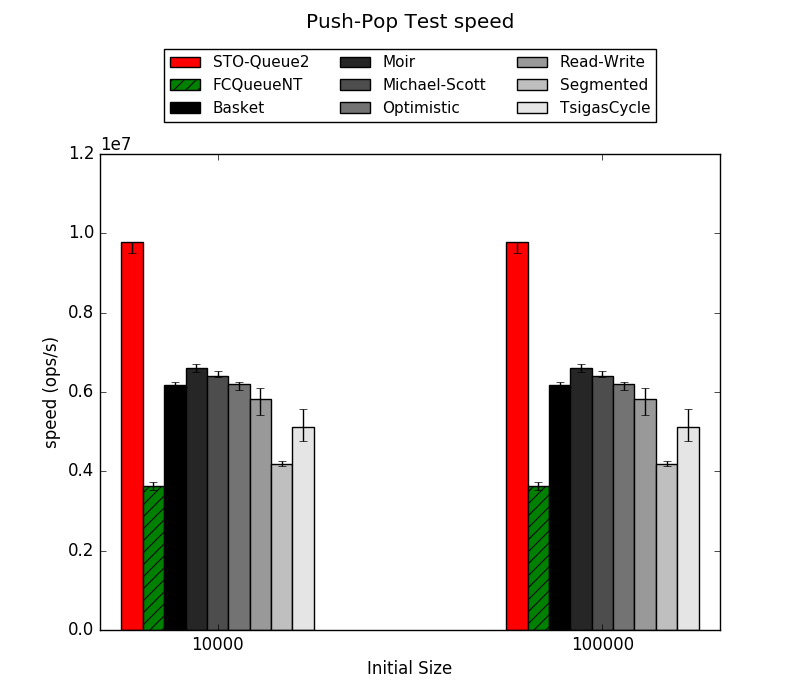
\includegraphics[height=3in]{concurrent/Q:PushPopspeed.png}
\caption{2-Thread Push-Pop Test Results of Various Concurrent Queues}
\label{fig:concurrent_queues}
\end{figure}

\paragraph{Multi-Thread Random Singleton Transactions Test}
\begin{figure}[ht!]
\centering
    \begin{minipage}{0.45\textwidth}
        \centering
        \includegraphics[height=2.5in]{concurrent/Q:RandSingleOps10000speed.png}
        \caption*{Initial Queue Size of 10000.\\Performance (ops/s) (higher is better)}
    \end{minipage}
    \begin{minipage}{0.45\textwidth}
        \centering
        \includegraphics[height=2.5in]{concurrent/Q:RandSingleOps100000speed.png}
        \caption*{Initial Queue Size of 100000.\\Performance (ops/s) (higher is better)}
    \end{minipage}
\caption{Multi-Thread Singletons Test Results of Various Flat-Combining and Transactional Queues}
\label{fig:concurrent_queues}
\end{figure}

Out of the concurrent data structures tested, the read-write queue\cite{queue1} and the flat combining queue consistently perform best on the 2-Thread Push-Pop Test. On the Multi-Thread Random Singleton Test, the flat combining queue achieves performance over $2.5\times$ greater than any other queue as the number of threads increases above 2.

For these reasons, as well as the algorithmic benefits of the flat combining technique described in Section~\ref{fcqueuent}, we focus our work on the flat combining queue.

We include the STO1 and STO2 queues in these benchmarks to measure the signficance of the gap between transactional and concurrent data structures. The STO queues---particularly the STO2 queue---outperform all but the read-write queue and flat combining queues on the 2-thread Push-Pop test. This test incurs the least contention and transactional overhead to track simply how fast the data structure can handle pushes and pops. It is unsurprising that, on this test, a simple synchronization strategy, such as that used in the STO queues, outperforms the majority of high-concurrency algorithms which are optimized for scalability. The Multi-Thread Random Singleton Transaction test demonstrate that as contention and transactional overhead (abort rate) increases, the flat combining queue maintains performance approximately 2.5$\times$ greater than that of the STO queues, although neither algorithm scales. However, the other high-concurrency algorithms appear to perform worse than our STO queues. We conjecture this may be due to the implementation of the algorithm used in our benchmarks\cite{libcds}.

\subsubsection{Flat Combining Queue Variants}

We benchmark several variants of the flat combining queue against our STO1 and STO2 queues. This includes:
\begin{itemize}
    \item FCQueueNT: the non-transactional flat combining queue.
    \item STO-FCQueue: the fully-transactional flat-combining queue.
    \item WrappedFCQueueNT: the non-transactional flat combining queue that invokes STO \texttt{start\_transaction} and \texttt{commit\_transaction} calls, but does not do any of the transactional bookkeeping necessary to provide transactional guarantees.
\end{itemize}

The relative performance of the WrappedFCQueueNT to the FCQueueNT indicates how much of the overhead added by the STO system is unavoidable (without modifications to STO itself). A data structure must always invoke the STO wrapper calls to support transactions. 

\paragraph{2-Thread Push-Pop Test}
\begin{figure}[ht!]
    \centering
    \begin{minipage}{0.45\textwidth}
    \centering
    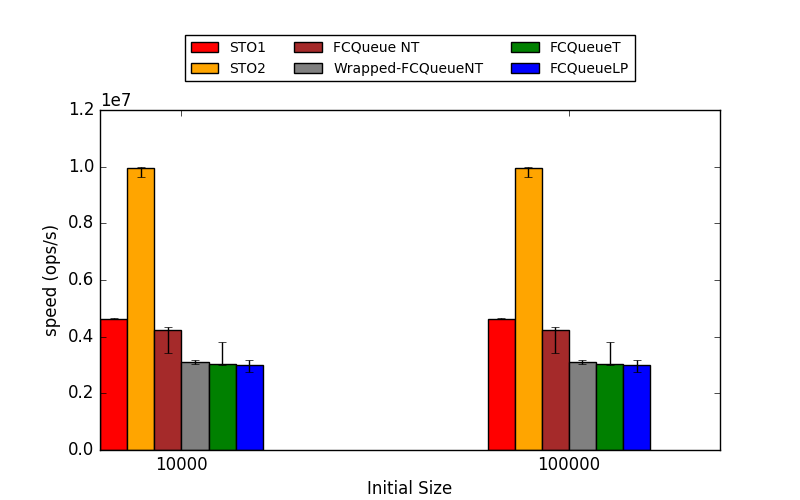
\includegraphics[height=2in]{fcqueues/Q:PushPopspeed.png}
    \caption*{Performance (ops/s)\\(higher is better)}
    \end{minipage}
    \begin{minipage}{0.45\textwidth}
    \centering
    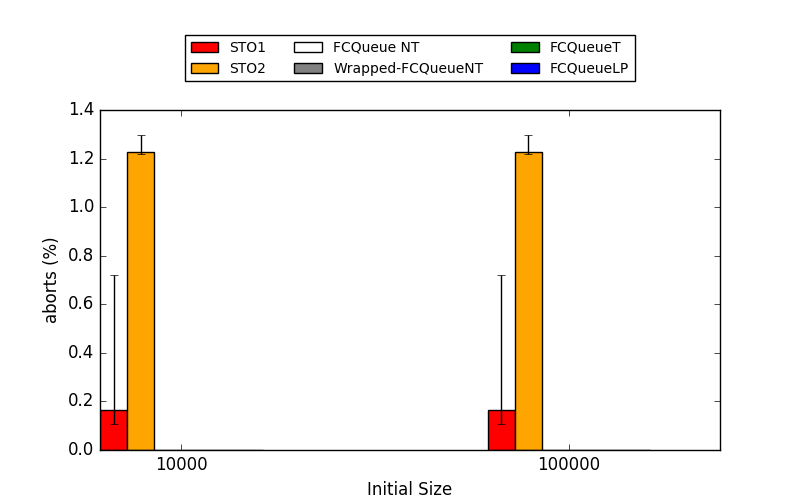
\includegraphics[height=2in]{fcqueues/Q:PushPopaborts.png}
    \caption*{\%Aborts\\(lower is better)}
    \end{minipage}
\caption{2-Thread Push-Pop Test Results of Various Flat-Combining and Transactional Queues}
\label{fig:fcqueues_queues}
\end{figure}

\paragraph{Multi-Thread Singletons Test}
\begin{figure}[ht!]
    \centering
    \begin{minipage}{0.45\textwidth}
    \centering
    \includegraphics[height=2.5in]{fcqueues/Q:RandSingleOps10000speed.png}
    \caption*{Initial Queue Size of 10000.\\Performance (ops/s) (higher is better)}
    \end{minipage}
    \begin{minipage}{0.45\textwidth}
    \centering
    \includegraphics[height=2.5in]{fcqueues/Q:RandSingleOps100000speed.png}
    \caption*{Initial Queue Size of 100000.\\Performance (ops/s) (higher is better)}
    \end{minipage}
    \\
    \begin{minipage}{0.45\textwidth}
    \centering
    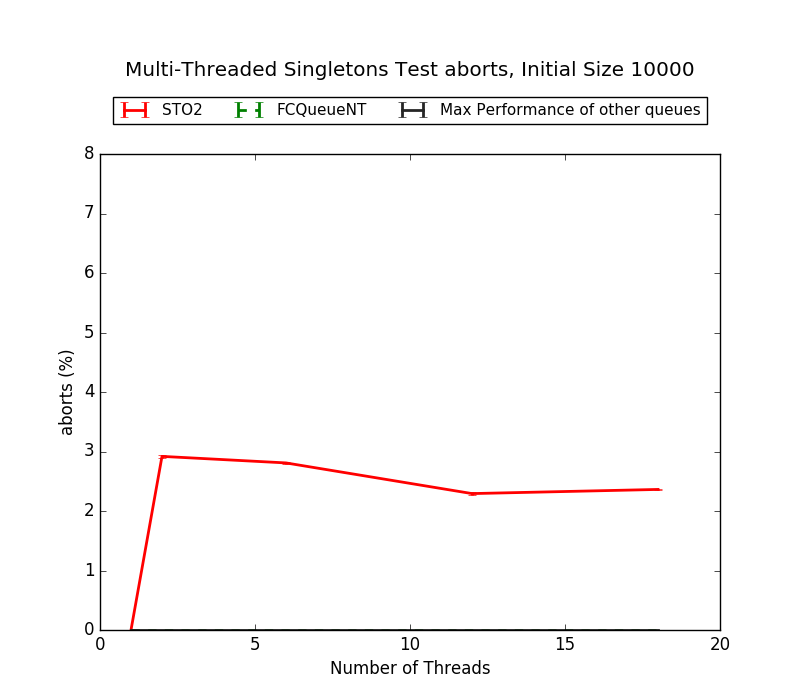
\includegraphics[height=2.5in]{fcqueues/Q:RandSingleOps10000aborts.png}
    \caption*{Initial Queue Size of 10000.\\\%Aborts (lower is better)}
    \end{minipage}
    \begin{minipage}{0.45\textwidth}
    \centering
    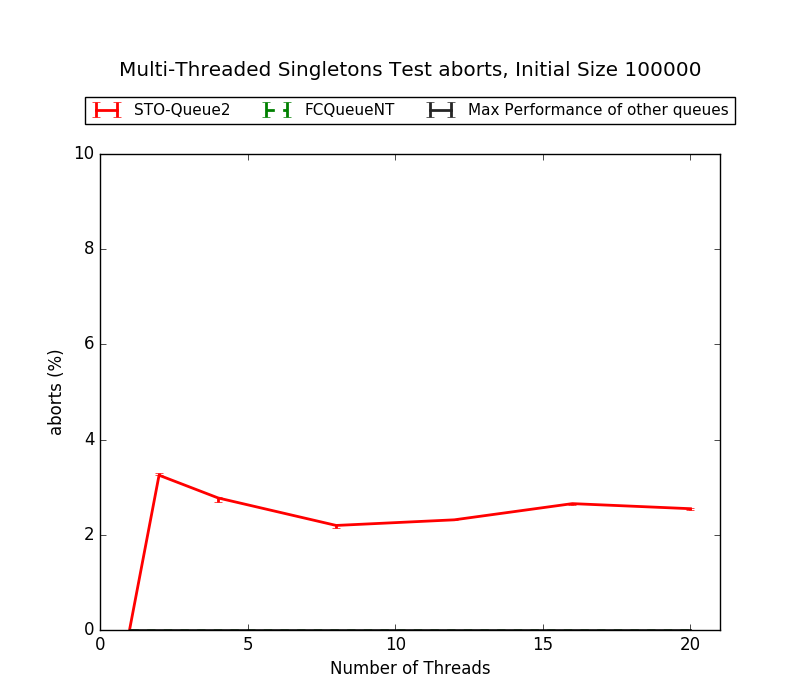
\includegraphics[height=2.5in]{fcqueues/Q:RandSingleOps100000aborts.png}
    \caption*{Initial Queue Size of 100000.\\\%Aborts (lower is better)}
    \end{minipage}
\caption{Multi-Thread Singletons Test Results of Various Flat-Combining and Transactional Queues}
\label{fig:txnal_queues}
\end{figure}


\section{Discussion}

\subsection{STO Overhead}
We first analyze what our results tell us about STO itself. Benchmarking transactional queues with naive concurrency algorithms (STO1 and STO2) against various high-concurrency algorithms demonstrates a simple implementation of a naive algorithm can consistently outperform more complex concurrent queue implementations even given the additional STO overhead. This indicates that the overhead added from STO does not cripple performance if used carefully---our transactional data structures can compete with several high-concurrency, non-transactional data structures. However, we see by comparing to the non-transactional flat combining queue that our algorithms are certainly not optimal for performance in a non-transactional setting.

Our comparison of the WrappedFCQueueNT and the FCQueueNT demonstrates that STO introduces some signficant necessary overhead \lyt{actual numbers here}. The STO wrapper calls (\texttt{start\_transaction} and \texttt{commit\_transaction}) allow a thread to mark which operations should occur together in the same transaction. After invoking the \texttt{start\_transaction} call, the thread can collect items in its read- and write-set; when \texttt{commit\_transaction} is invoked, the commit procedure is run (validation and installation of items in the read-/write-sets). The WrappedFCQueueNT adds no items to the read-/write-sets after invoking \texttt{start\_transaction}, and therefore incurs the minimum amount of overhead necessary to use STO:\ the commit procedure has zero items to validate or install. The WrappedFCQueueNT therefore represents the upper bound of performance we can expect from our STO queues. Even with the wraper calls, our results indicate it can still be possible to achieve performance \lyt{numbers} times greater than that of our original STO1 and STO2 queues.

\subsection{Transactional Flat Combining Queue}

Our results for the flat combining queue variants indicate that the fully-transactional flat combining queue algorithm (STO-FCQueue) performs poorly. Analysis with the \texttt{perf} tool indicates that the majority of the overhead is incurred from spinning on the flat combining lock (acquired by the combiner thread) or waiting for a flat combining call to complete. We see these results because of two reasons:
\begin{enumerate}
\item \emph{Higher Quantity}: A thread must make multiple flat combining calls to perform a pop within a transaction (recall that a push only requires one flat combining call) 
\item \emph{Higher Complexity}: each flat combining call requires executing instructions, which makes each operation request more expensive.
\end{enumerate}

We conclude that the flat combining technique, while perhaps near-optimal for a highly-concurrent data structure, is no better in a transactional setting than a naive synchronization technique such as that used in the STO1 and STO2 queues. This is because the flat combining algorithm must track the transaction state (e.g., going to perform two pops, one of which observes an empty queue) in order to provide transactional guarantees. In the next chapter, we formalize this argument using a commutativity discussion and claim that the higher quantity of more complex flat combining calls is necessary for flat combining to be used in a transactional setting: the flat combining technique depends on operation commutativity present in only a non-transactional setting to achieve its high performance. 



\chapter{HashMap Algorithms and Analysis}
\label{HashMap}

This chapter investigates different concurrent and transactional algorithms for hashmaps. We begin with an overview of concurrent and transactional hashmap specifications and algorithms. We then evaluate how these hashmaps perform on several microbenchmarks, and discuss why and how particular high-concurrency hashmap algorithms, modified to provide transactional guarantees, can outperform our current transactional algorithms.

\section{Algorithms}

We present the concurrency and transactional algorithms we analyzed, created, and implemented in our work. Some general terminology: an \emph{element} refers to the key-value pair inserted into the hashmap. A \emph{bucket} is a container of elements, and a hashmap consists of a set of buckets. The algorithms differ in the methods used to place elements in buckets and track how buckets and elements are modified.

\subsection{STO Chaining HashMap}
The STO Chaining HashMap (ChainingHashmap) is a concurrent, transactional hashmap implemented using a standard chaining algorithm. If two elements are mapped to the same bucket, they are chained in a linked list. Thus, the worst case lookup/delete is $O(n)$. Inserts are always constant time and require allocating an element. Each bucket is associated with a \emph{bucketversion} that increments upon any committed addition or removal from the bucket. The bucketversion is used to verify that no thread has added an element that was absent during a transaction's find. In addition, each bucket has a lock that synchronizes access to the bucket. Each inserted element is associated with an \emph{elementversion} that tracks if the value to the element has been modified or if the element has been removed.

Elements are inserted at execution time but marked as \emph{phantom}, allowing another transaction that sees ones of these uninstalled elements to realize it is viewing an inconsistent state of the map and therefore abort. If a transaction containing insertions aborts, these phantom elements are removed from the map. ELse thephantom mark is erased during commit. An alternative approach would be to insert all elements at commit time.However, this requires either relying on the bucketversion to determine if another transaction has inserted the same element (which would result in false aborts since the bucketversion increments for \emph{any} inserted value) or redoing the search for the element to see if the insertion can still occur. Thus, we insert at execution time to allow for more fine-grained validation checks at commit time and to reduce redundant computations. Deletions are delayed until commit time (an optimistic approach). This requires careful handling of cases of \emph{read\_my\_writes}, such as deleting an element inserted in the same transaction, 

\subsection{Non-Transactional Cuckoo HashMap}
The Non-Transactional Cuckoo HashMap (CuckooHashMapNT) implements a concurrent, non-transactional cuckoo hashing algorithm (implementation modified from \cite{cuckoocode}).

Each element is placed in one of two buckets; these buckets are determined by two different hash functions. A bucket has a fixed size of elements. This means that lookups and deletes only require executing two hash functions and checking the contents of two buckets (an $O(1)$ operation).

Inserts run in amortized time $O(1)$ but may occasionally be $O(n)$.
If an element $e$ is hashed by the first hash function to a bucket that is already full, the algorithm attempts to place $e$ in its alternative bucket by hashing $e$ with the second hash function. If both buckets are full, cuckoo shuffling occurs. This process kicks out an element $e'$ in one of $e$'s buckets and places $e'$ in $e'$'s alternative bucket. If $e'$'s alternative bucket is full, an element $e''$ is ejected from this bucket, and so on. As long as the cuckoo shuffling does not encounter a bucket cycle, $e$ can now be placed in one of its buckets, as the removal of $e'$ has made space for $e$.
However, if the shuffling encounters a bucket cycle, the hashmap raises an \texttt{out of space} assertion error. We can imagine an alternative implementation that allows the hashmap to grow in number of buckets or otherwise change its hash functions, reinserting all elements, but for simplicity, we keep the algorithm statically sized.

Because the buckets are statically sized, elements are contained in fixed-size key and value arrays and therefore do not require extra allocations.

\subsection{STO CuckooHashMap}
The STO CuckooHashMap comes in three flavors: allocating, allocating with key-fragments, and non-allocating. All flavors instrument the non-transactional cuckoo hashmap with STO calls that provide transactional guarantees.
Both allocating and non-allocating versions use the same synchronization algorithm: like the STO Chaining HashMap, each bucket has a \emph{bucketversion} and lock and each element has an \emph{elementversion}. Because insertions can occur due to cuckoo shuffling as well as an external insertion call, the bucketversion increments only when an element \emph{not already contained in the map} is inserted into the bucket (i.e., elements inserted via a call to insert and not via cuckoo shuffling). Elements are inserted at execution time with a \emph{phantom} flag that is then erased at commit time, and deletions are delayed until commit time.

The allocating STO CuckooHashMaps allocate elements upon insertion, with buckets containing pointers to the elements. This allows STO to track elements by their memory address to verify elementversions at commit time. The key-fragments variant expands buckets to contain both an array of keys and an array of element pointers. This enables a lookup or delete for an absent item to skip following the pointer to the allocated internal element itself, and can reduce the number of cache line accesses depending on the workload.

The non-allocating STO CuckooHashMap consists of buckets consisting of a fixed-sized array of wrapped elements. STO tracks elements by their keys. Therefore, to verify if an elementversion has changed at commit time, the check procedure performs a find of the element using the key (searching at most two buckets) and validates the corresponding elementversion. Although this reduces the number of allocations, elementversions can now move between buckets, and the values in their previous locations invalidated. This complicates correctly checking and synchronizing the reads of elementversions.

\section{Evaluation}

\subsection{Microbenchmarks}
As with the queue, all hashmaps queues are evaluated on a set of microbenchmarks to demonstrate their scalability and performance. The controlled nature of these microbenchmarks allow us to easily compare particular aspects of each algorithm, such as transactional overhead introduced by STO. All experiments are run on the same machine as the queue experiments (with 100GB DRAM, two 6-core Intel Xeon X5690 processors with hyperthreading clocked at 3.47GHz and a 64-bit Linux 3.2.0 operating system). All benchmarks and STO data structures are compiled with g++-5.3. In all graphs, we show the median of 5 consecutive runs with the minimum and maximum performance results represented as error bars.

\subsubsection{Parameters}

\begin{itemize}
    \item Proportion of Finds/Inserts/Deletes: The ratio of inserts:deletes is kept at 1 to ensure that the hashmap does not always become empty or only grow in size. It is expected that half the inserts will succeed and half the deletes will succeed, since both are drawing key values from the same range. Tests of 5\% inserts, 5\% deletes, and 90\% finds simulate the most likely use cases for hashmaps\cite{hm1}. Tests of equal proportion (33\%) of all operations investigate how the hashmap reacts to an increased rate of inserts and deletes.
    \item Maximum Key Value: The max key value of inserted elements is twice the number of elements the hashmap will contain when it reaches a fixed point for its size. Thus, altering the maximum value changes the load on the hashmap
    \item Operations per transaction: We choose to run all tests comparing transactional to non-transactional (parallel-only) data structures using single-operation transactions. As discussed in Section~\ref{q_microbenchmarks}, this provides a more fair evaluation of transactional data structures against concurrent ones. In addition, it allows us to minimize the differences between transaction hashmap implementations so we can get a baseline comparison.
    \item Capacity: the number of buckets $\times$ the number of items per bucket. With the Chaining hashmap, capacity is infinite (within memory constraints) because buckets can grow arbitrarily large. The CuckooHashMaps have a fixed size bucket, and therefore a finite capacity. 
        The number of buckets and the size of each bucket affects the number of cache lines accessed during the test (for example, a larger hashmap may not be expected to fit into the L2 cache, whereas a small hashmap at full capacity will fit entirely in cache). During all tests, the number of keys present in the hashmap is not allowed to outgrow its capacity.
    \item Load: The number of keys : capacity ratio. This determines the average length of chains in a chaining hashmap and the average number of items to be found per bucket. At steady state, load is expected to be half of maximum load. 
\end{itemize}
Note that the initial size of the data structure should not affect performance as the test proceeds for a longer period of time and reaches a steady state. Therefore, we do not include the initial size as a benchmark parameter.

\subsubsection{Multi-Thread, Variable-Capacity Singletons Test} 
This test is run with different numbers of threads and with different proportions of finds/inserts/deletes. Each thread runs 5 million singleton transactions.
The test is run twice, once with a probability of 33\% insert, 33\% delete, and 34\% find, and again with a probability of 5\% insert, 5\% delete, and 90\% find. The steady-state final size is 50\% maximum load.

\subsection{Results and Discussion}

We measure all hashmap's performance in terms of operations per second, abort rates, and cache performance (number of cache misses). 

\begin{figure}[h!]
    \centering
    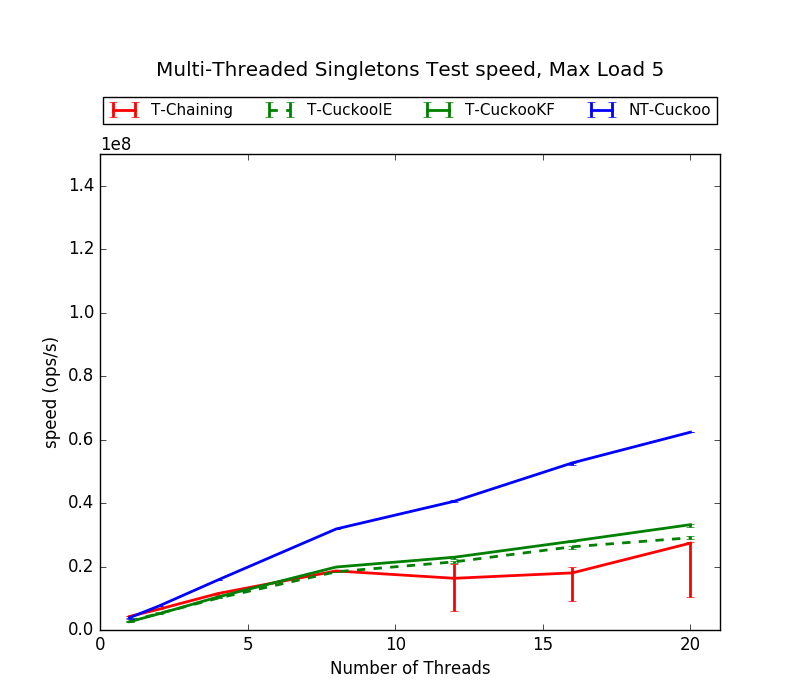
\includegraphics[height=2in]{maps/5HM1M:F34,I33,E33speed.png}
    $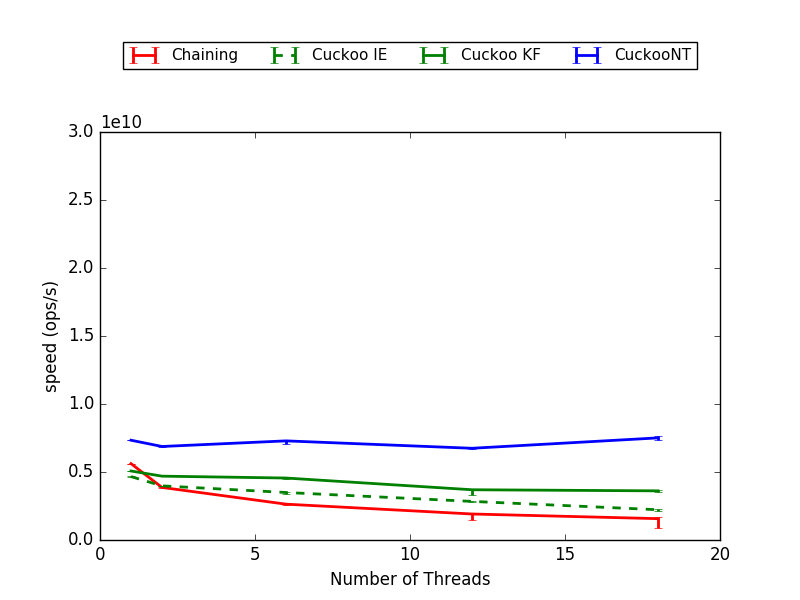
\includegraphics[height=2in]{maps/10HM1M:F34,I33,E33speed.png}
    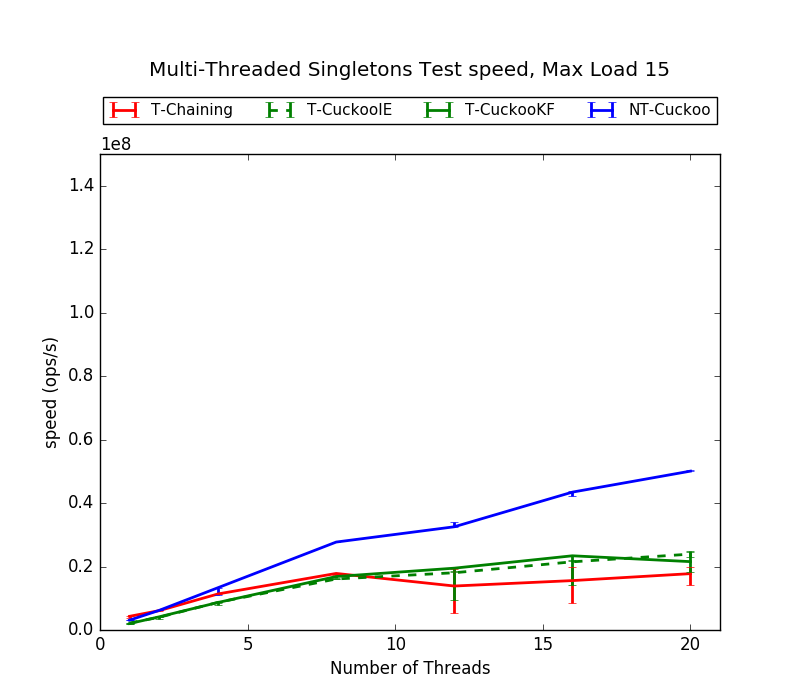
\includegraphics[height=2in]{maps/15HM1M:F34,I33,E33speed.png}
    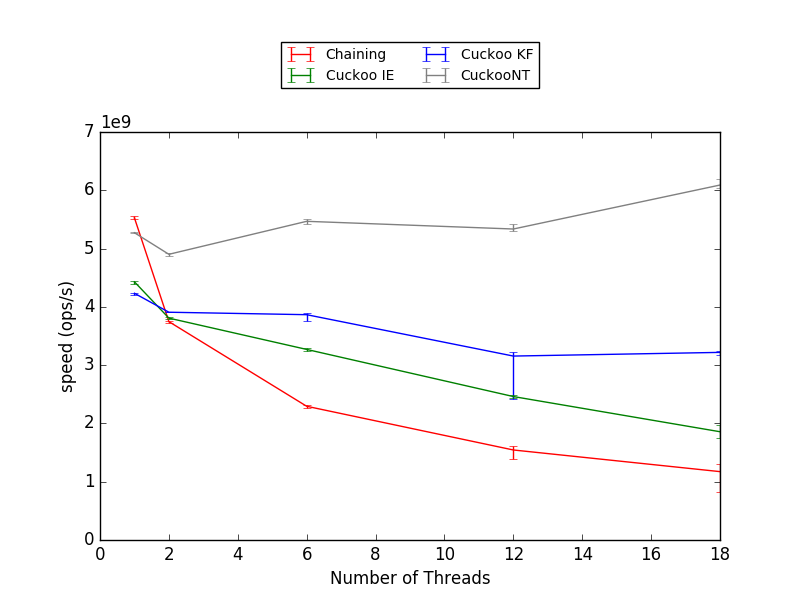
\includegraphics[height=2in]{maps/20HM1M:F34,I33,E33speed.png}
    \\
    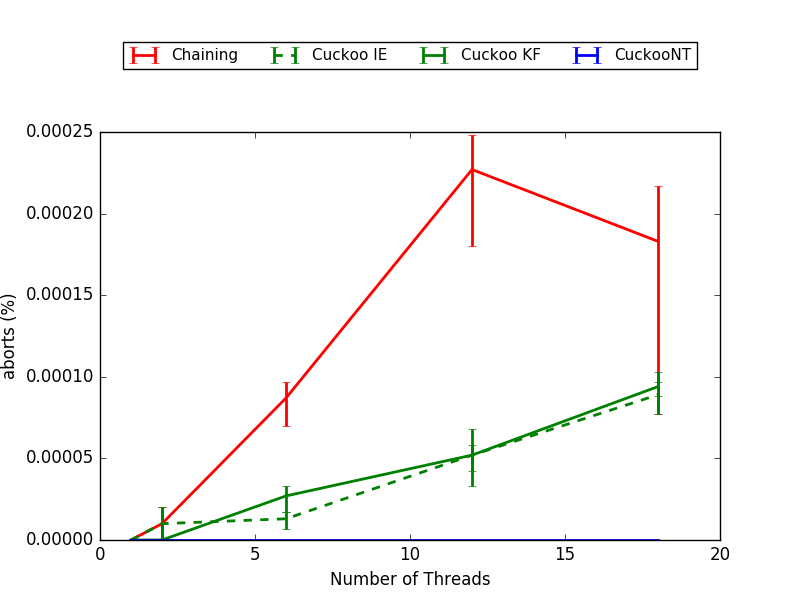
\includegraphics[height=2in]{maps/5HM1M:F34,I33,E33aborts.png}
    $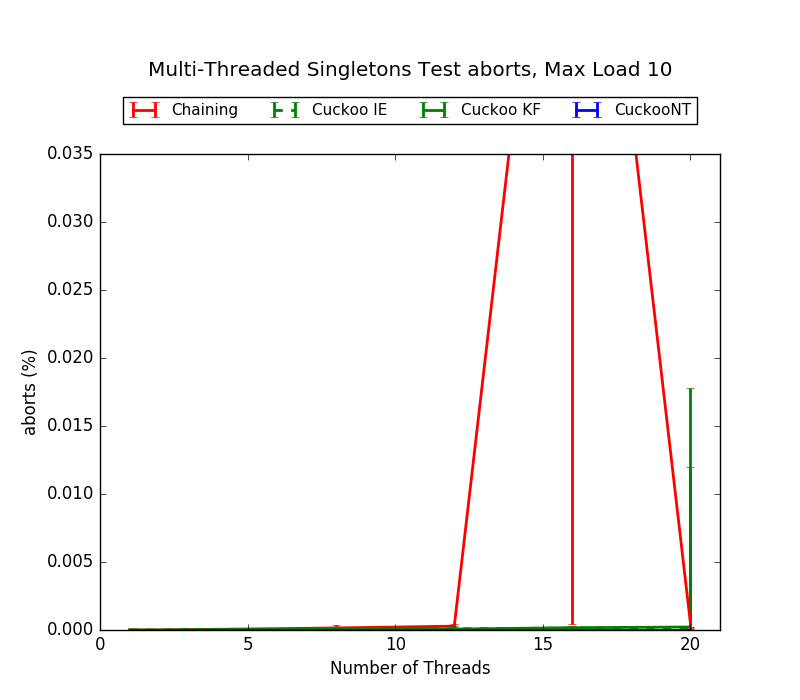
\includegraphics[height=2in]{maps/10HM1M:F34,I33,E33aborts.png}
    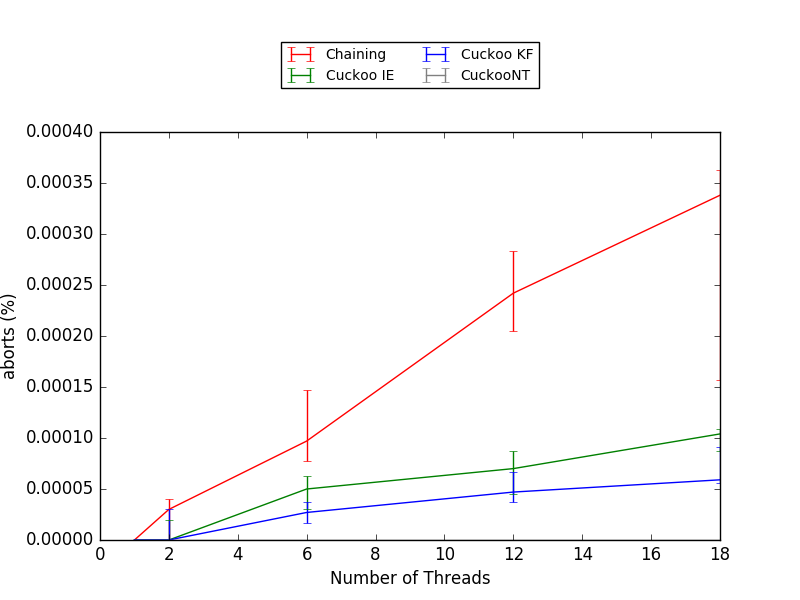
\includegraphics[height=2in]{maps/15HM1M:F34,I33,E33aborts.png}
    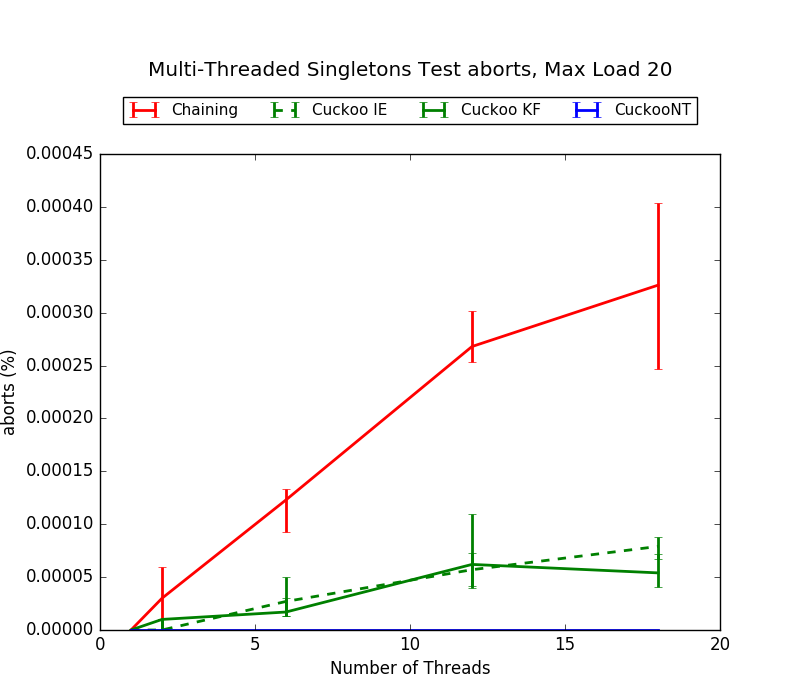
\includegraphics[height=2in]{maps/20HM1M:F34,I33,E33aborts.png}
    \\
    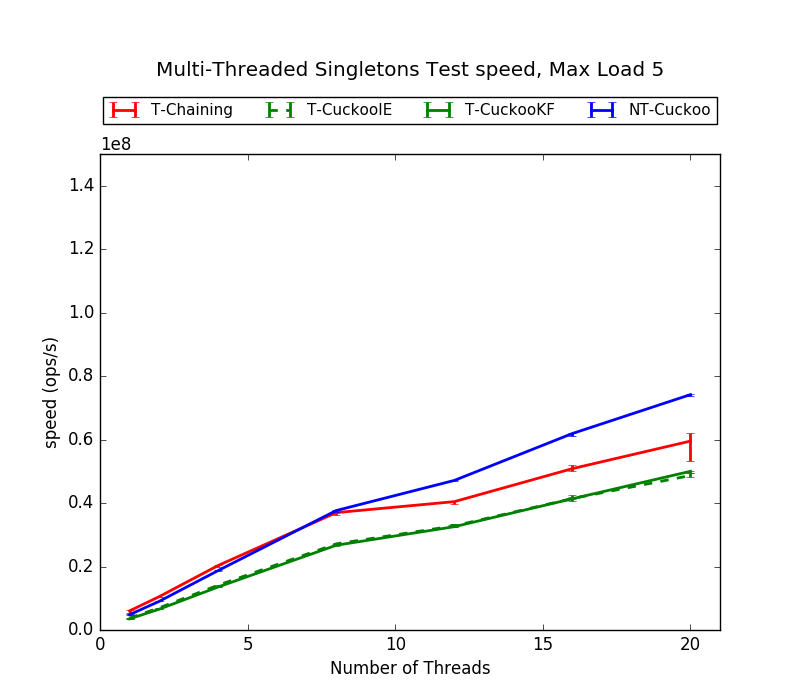
\includegraphics[height=2in]{maps/5HM1M:F90,I5,E5speed.png}
    $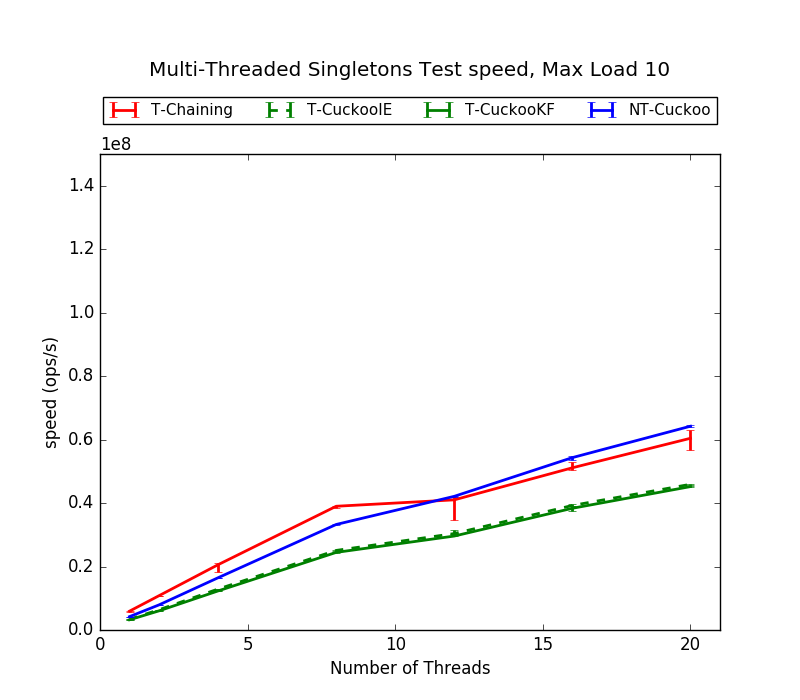
\includegraphics[height=2in]{maps/10HM1M:F90,I5,E5speed.png}
    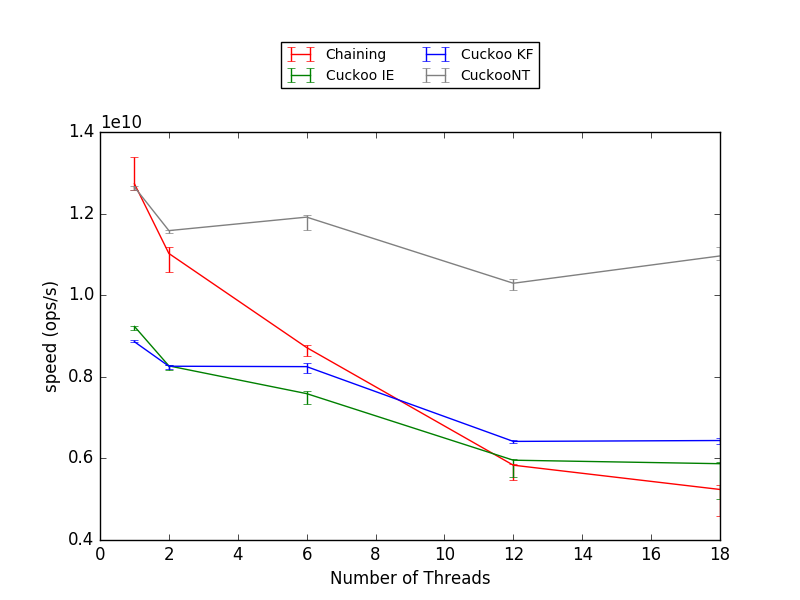
\includegraphics[height=2in]{maps/15HM1M:F90,I5,E5speed.png}
    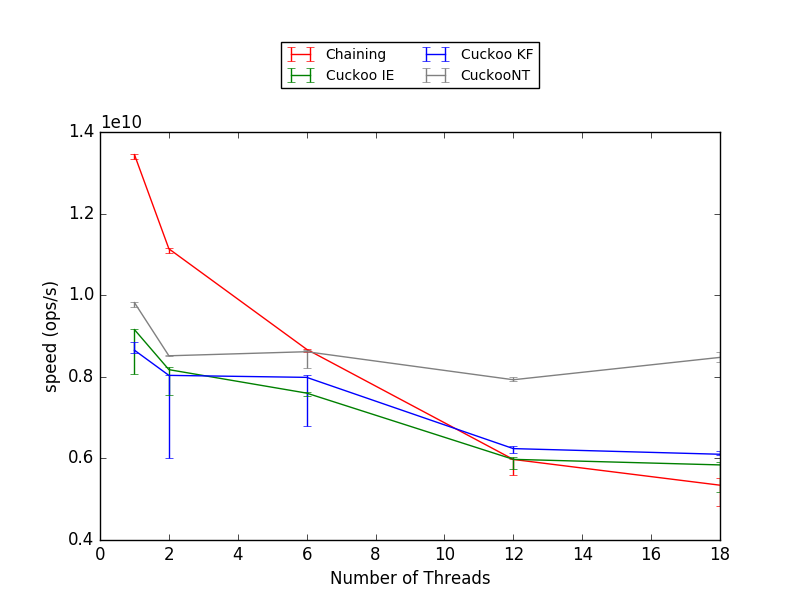
\includegraphics[height=2in]{maps/20HM1M:F90,I5,E5speed.png}
    \\
    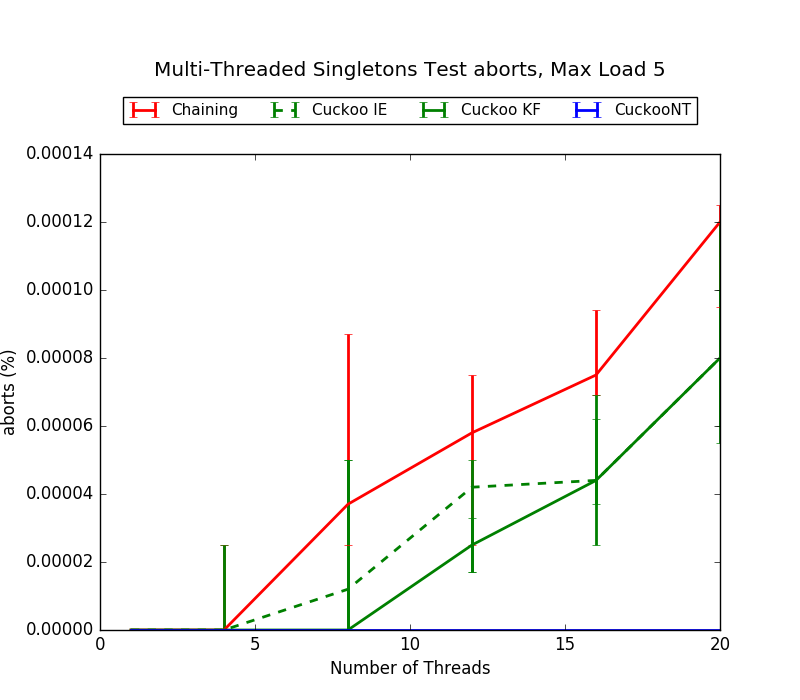
\includegraphics[height=2in]{maps/5HM1M:F90,I5,E5aborts.png}
    $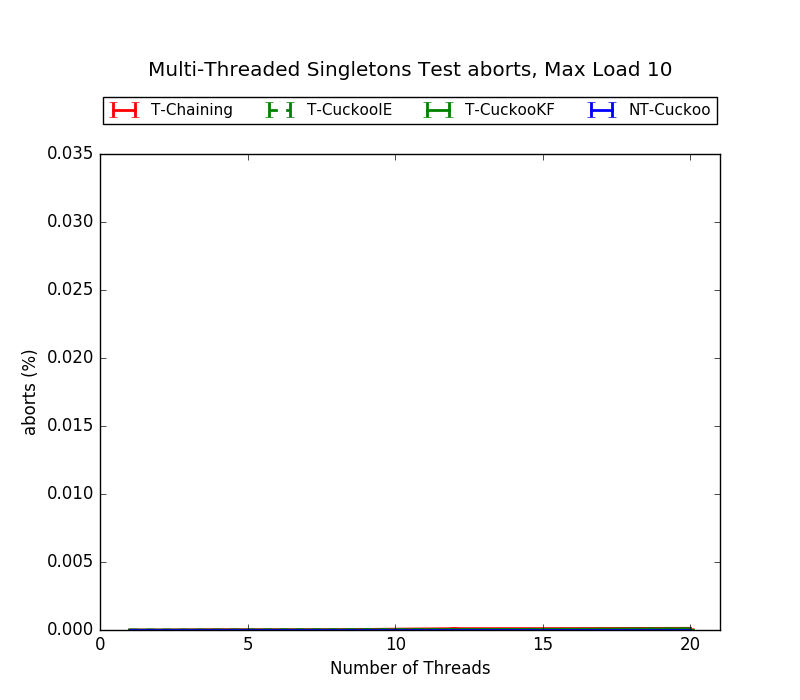
\includegraphics[height=2in]{maps/10HM1M:F90,I5,E5aborts.png}
    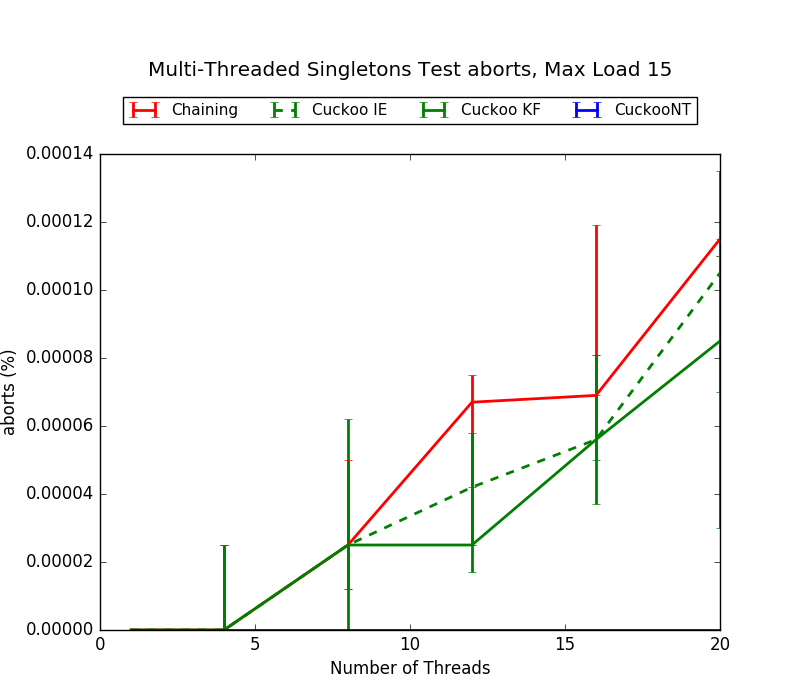
\includegraphics[height=2in]{maps/15HM1M:F90,I5,E5aborts.png}
    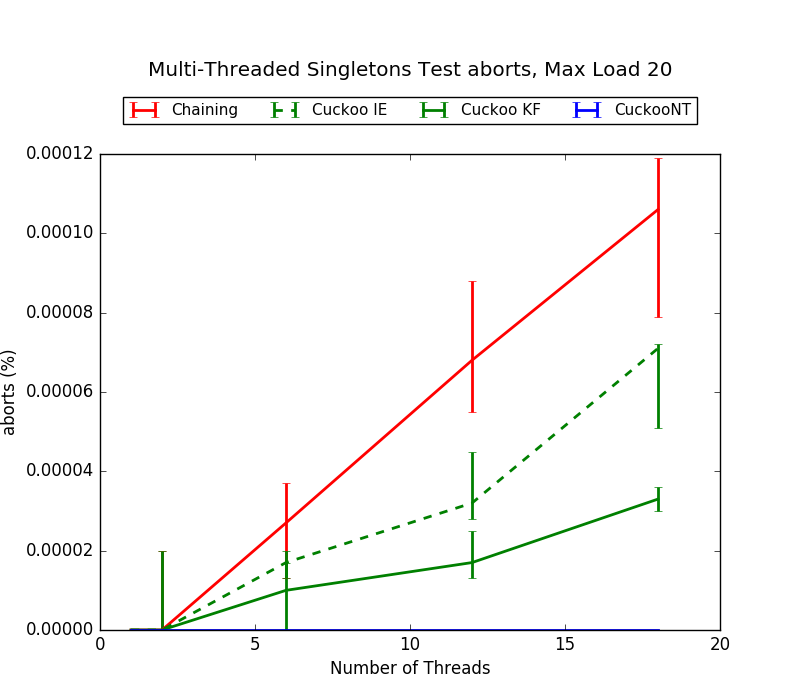
\includegraphics[height=2in]{maps/20HM1M:F90,I5,E5aborts.png}
\caption{Hashmap with 1 Million Buckets}
\label{fig:ntqueues}
\end{figure}

\begin{figure}[h!]
    \centering
    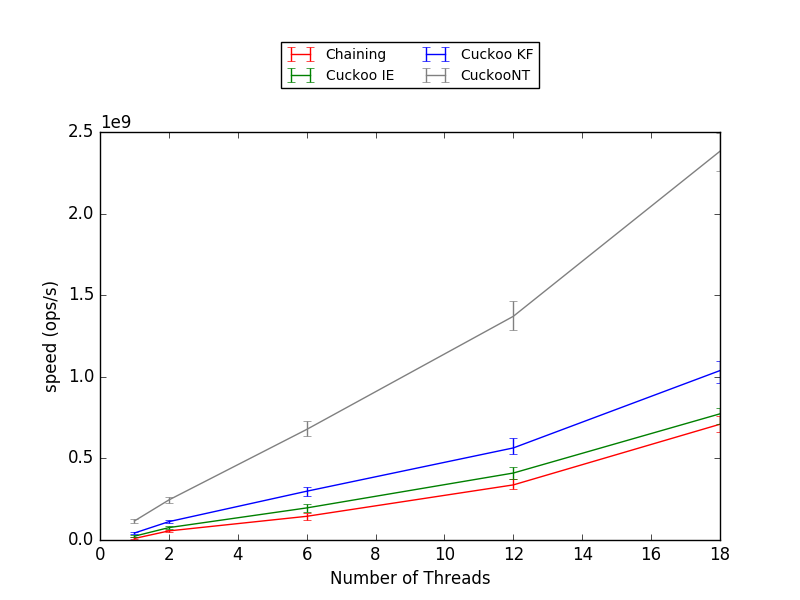
\includegraphics[height=2in]{maps/5HM125K:F34,I33,E33speed.png}
    $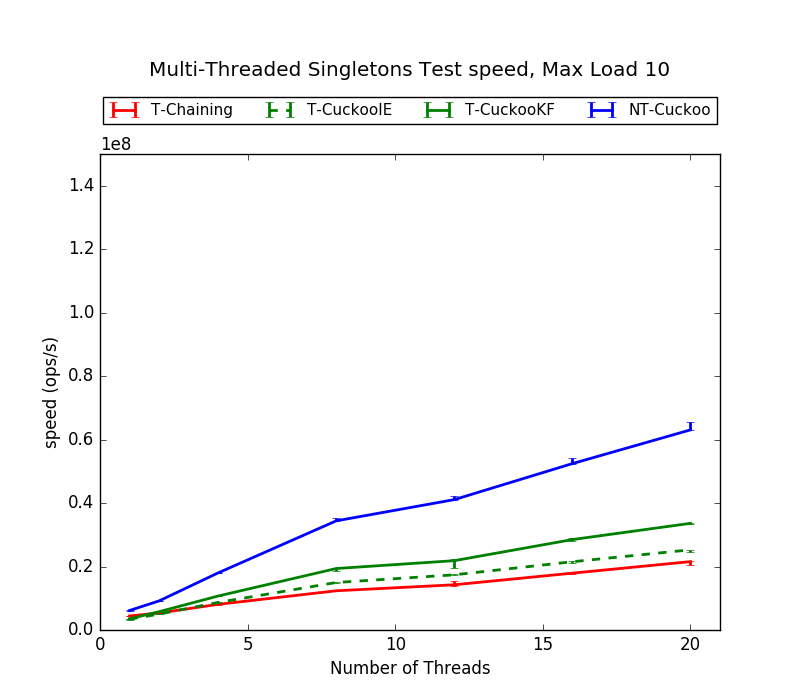
\includegraphics[height=2in]{maps/10HM125K:F34,I33,E33speed.png}
    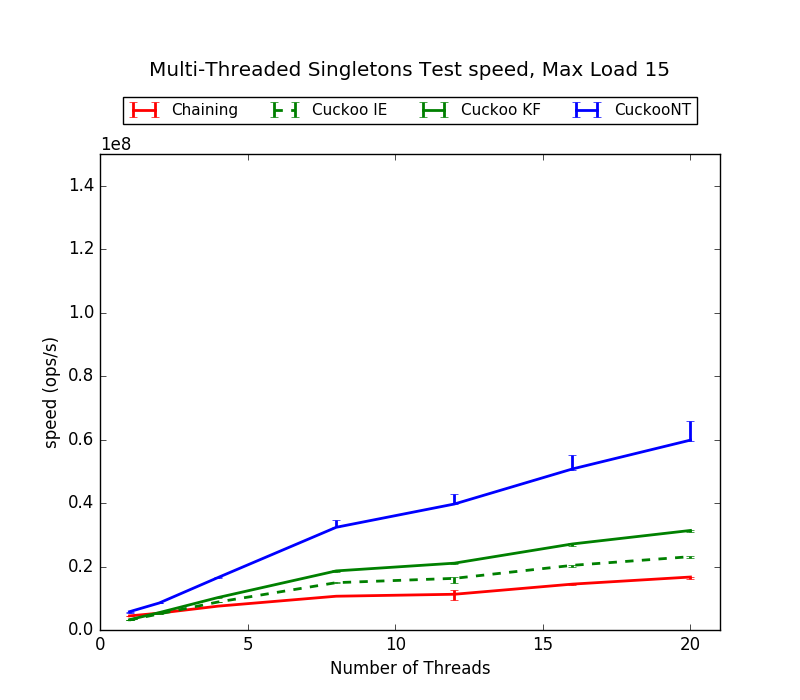
\includegraphics[height=2in]{maps/15HM125K:F34,I33,E33speed.png}
    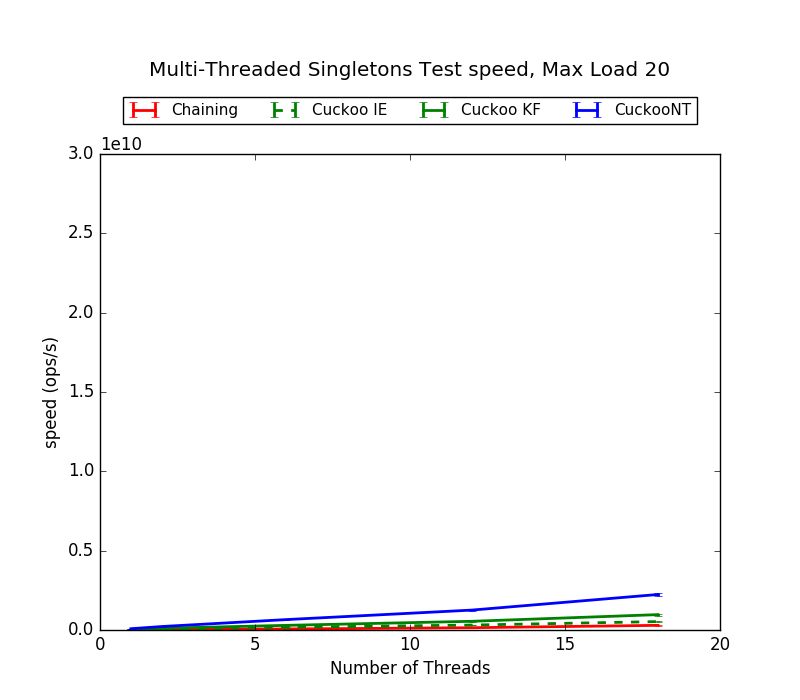
\includegraphics[height=2in]{maps/20HM125K:F34,I33,E33speed.png}
    \\
    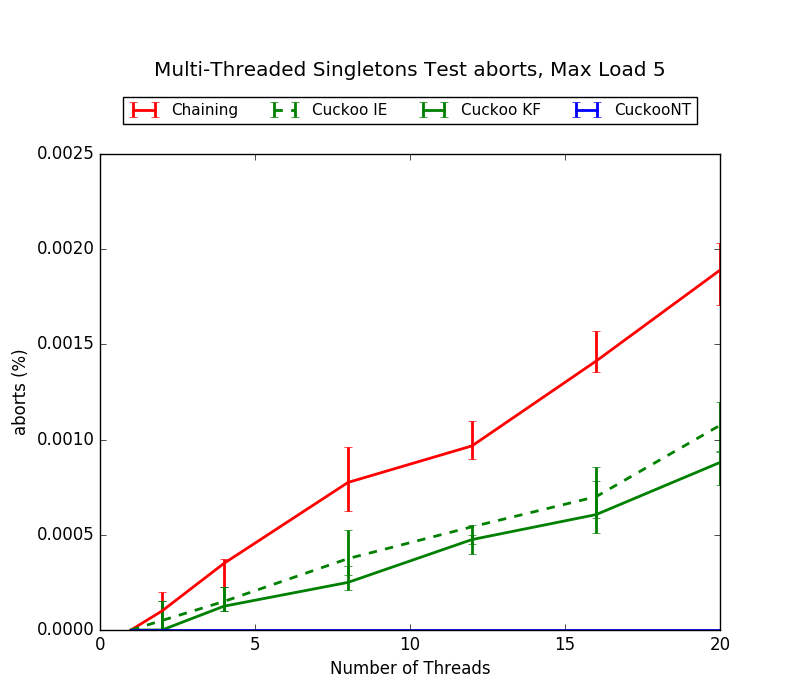
\includegraphics[height=2in]{maps/5HM125K:F34,I33,E33aborts.png}
    $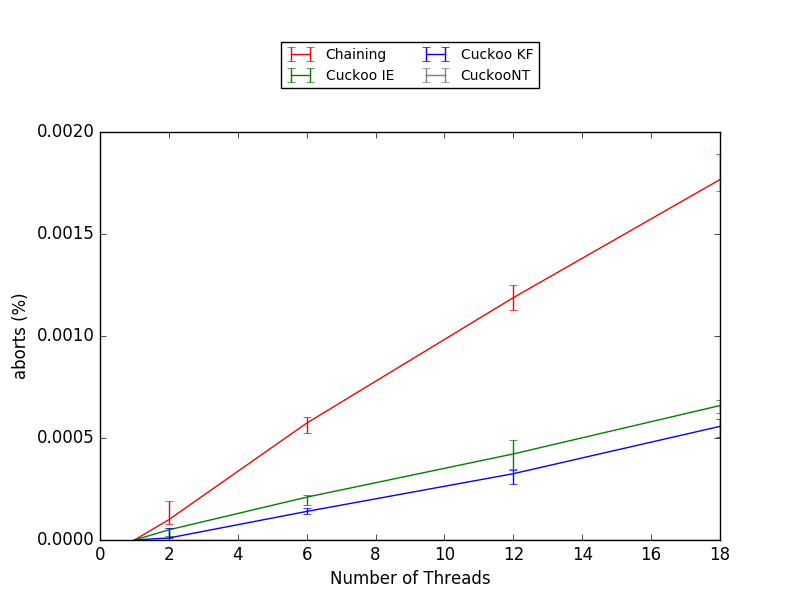
\includegraphics[height=2in]{maps/10HM125K:F34,I33,E33aborts.png}
    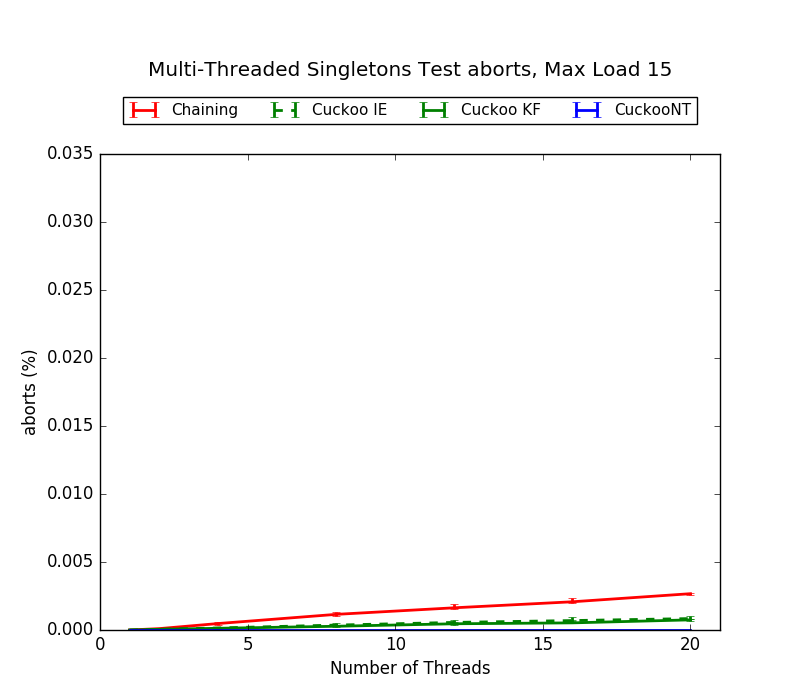
\includegraphics[height=2in]{maps/15HM125K:F34,I33,E33aborts.png}
    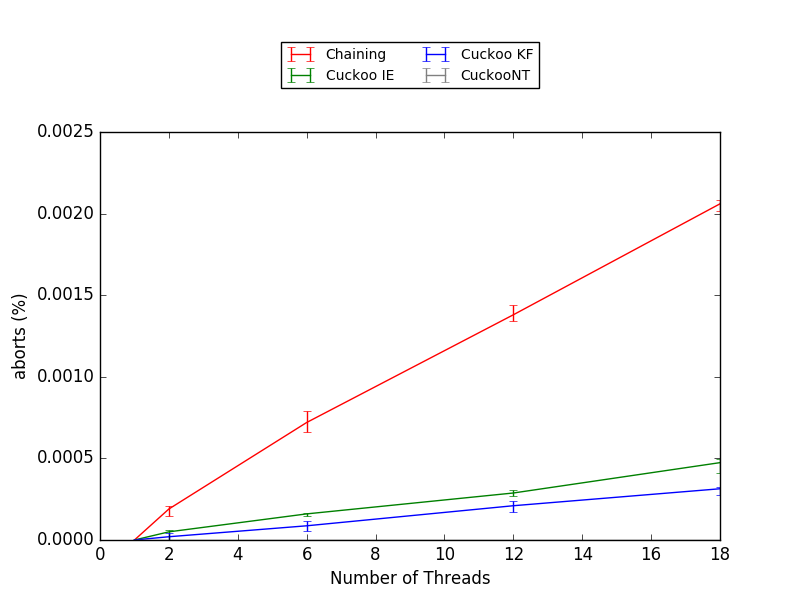
\includegraphics[height=2in]{maps/20HM125K:F34,I33,E33aborts.png}
    \\
    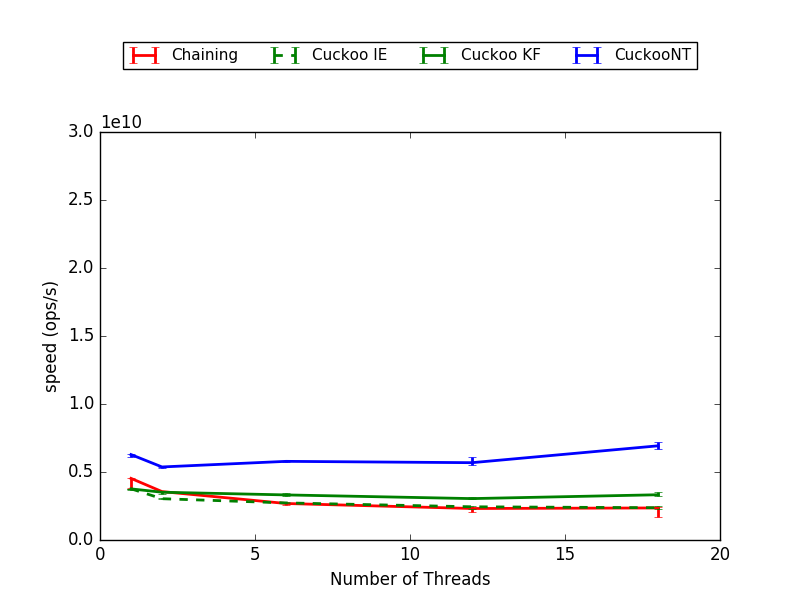
\includegraphics[height=2in]{maps/5HM125K:F90,I5,E5speed.png}
    $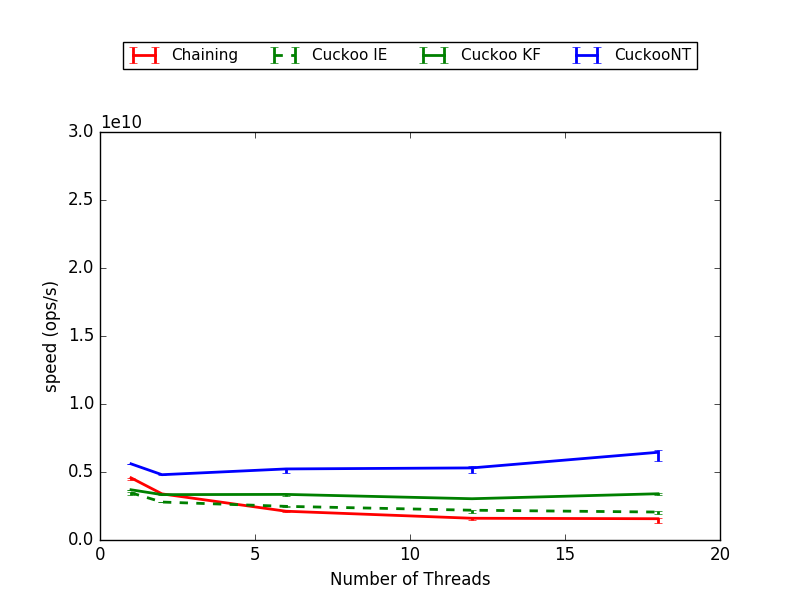
\includegraphics[height=2in]{maps/10HM125K:F90,I5,E5speed.png}
    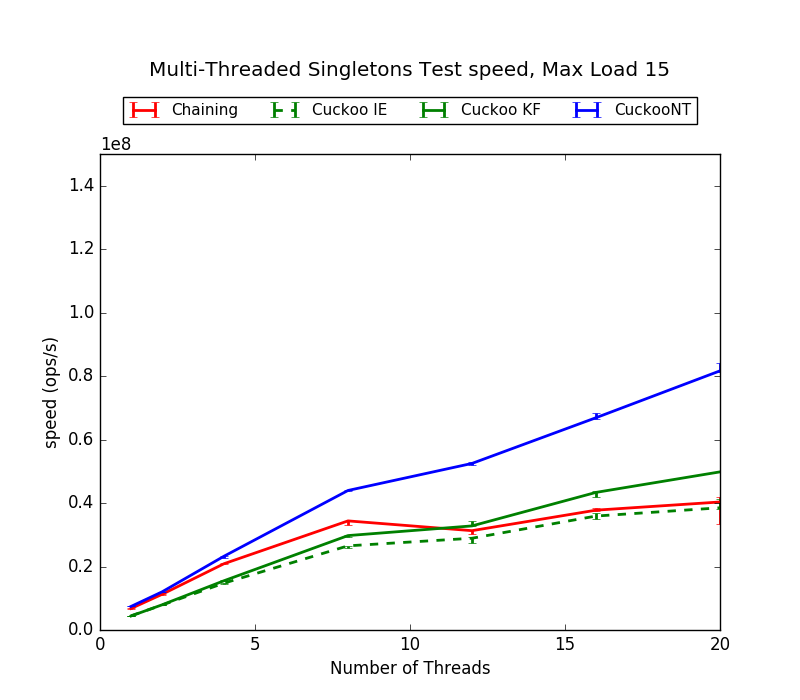
\includegraphics[height=2in]{maps/15HM125K:F90,I5,E5speed.png}
    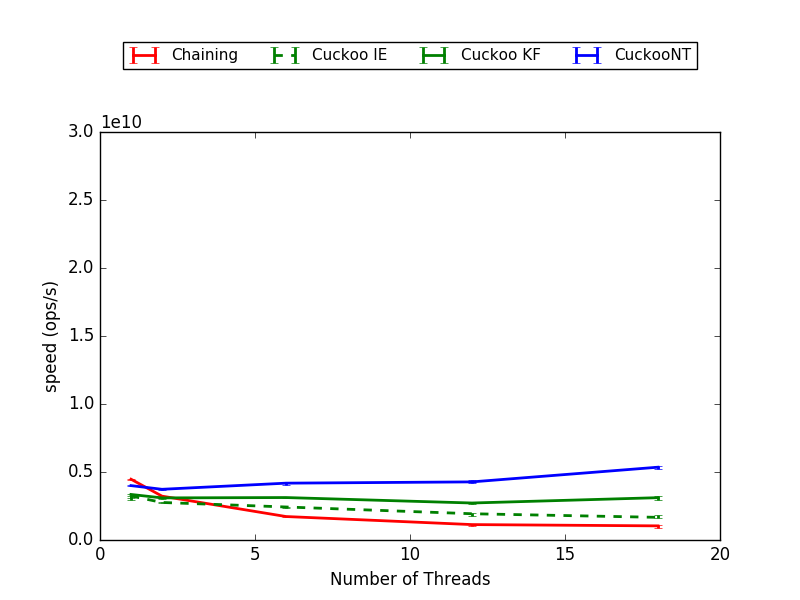
\includegraphics[height=2in]{maps/20HM125K:F90,I5,E5speed.png}
    \\
    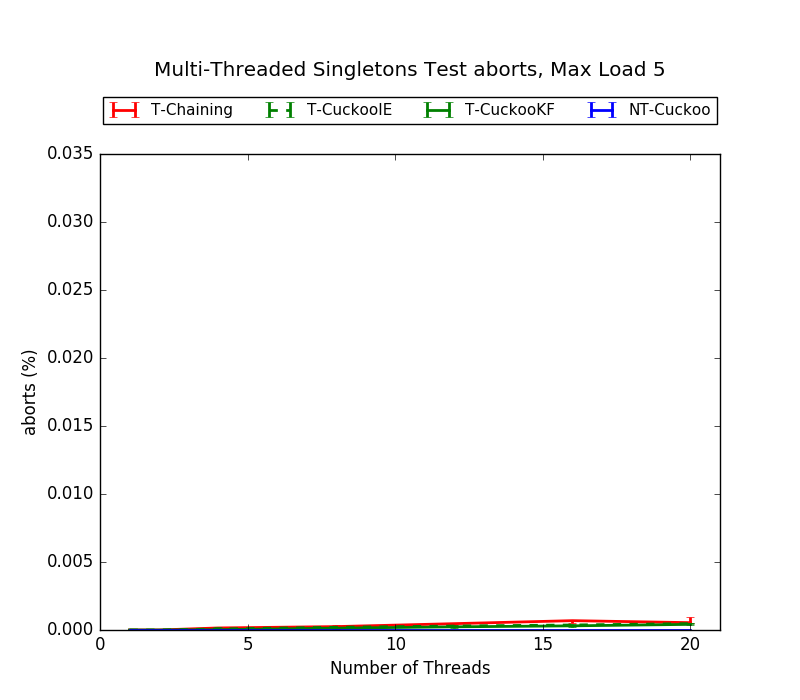
\includegraphics[height=2in]{maps/5HM125K:F90,I5,E5aborts.png}
    $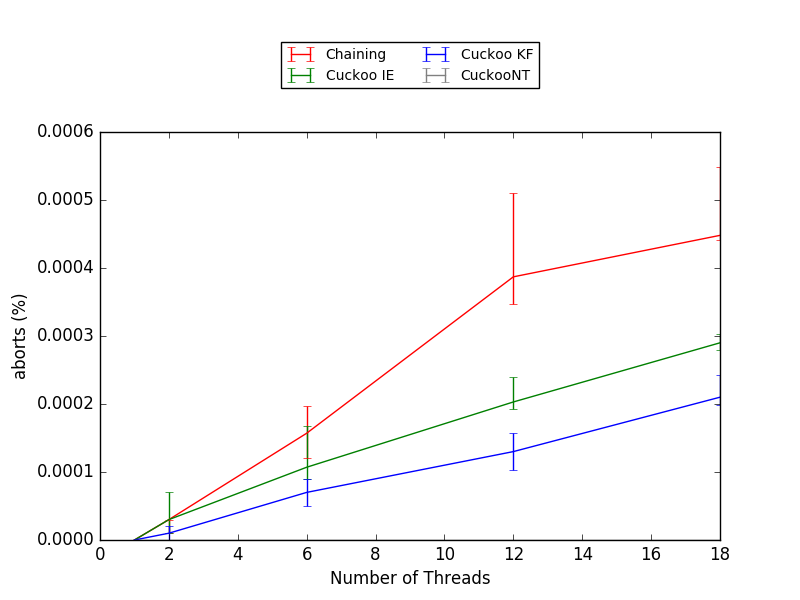
\includegraphics[height=2in]{maps/10HM125K:F90,I5,E5aborts.png}
    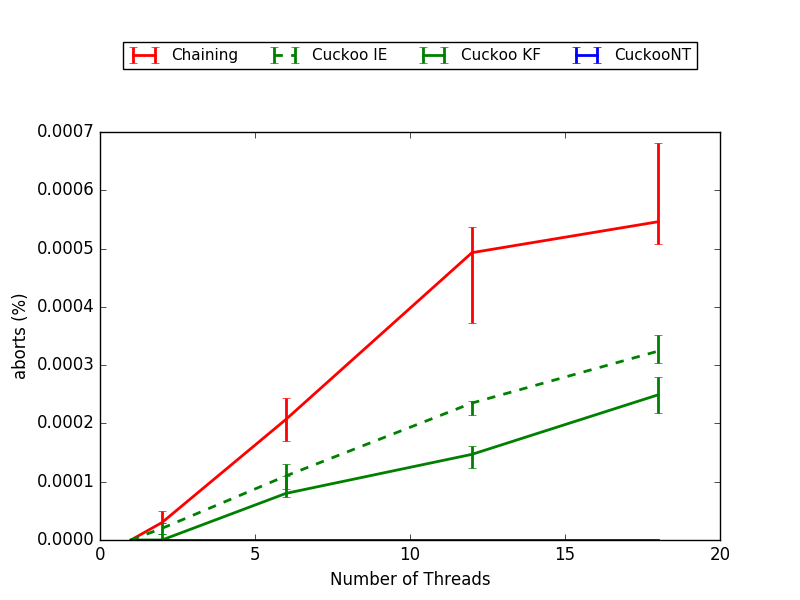
\includegraphics[height=2in]{maps/15HM125K:F90,I5,E5aborts.png}
    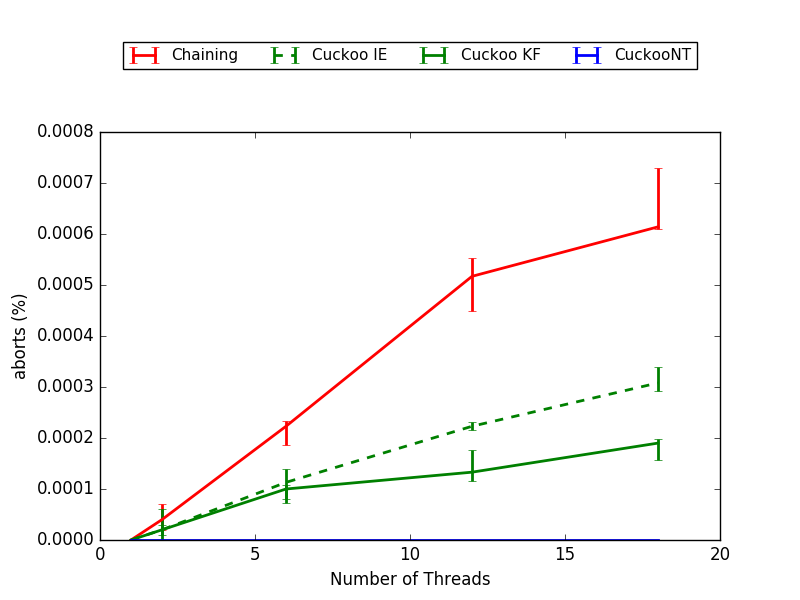
\includegraphics[height=2in]{maps/20HM125K:F90,I5,E5aborts.png}
\caption{Hashmap with 125K Million Buckets}
\label{fig:ntqueues}
\end{figure}

\begin{figure}[h!]
    \centering
    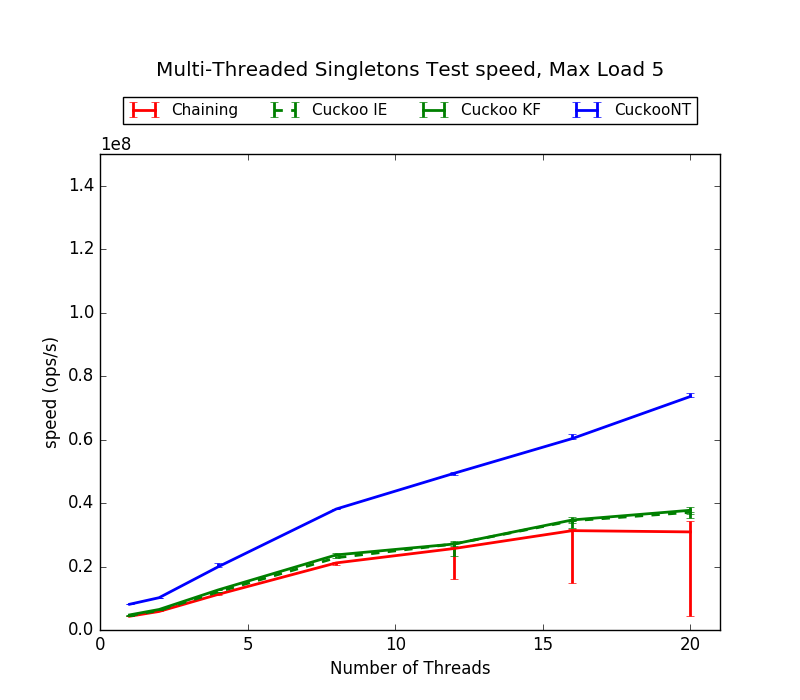
\includegraphics[height=2in]{maps/5HM10K:F34,I33,E33speed.png}
    $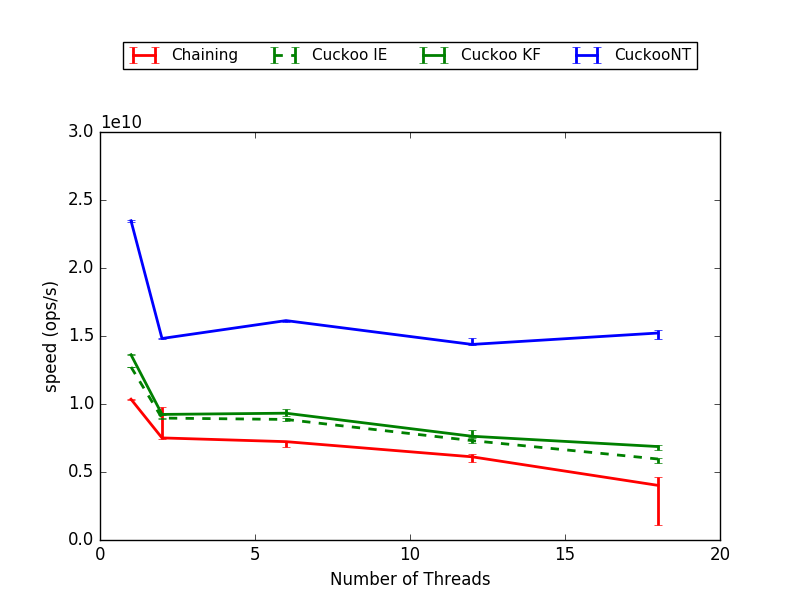
\includegraphics[height=2in]{maps/10HM10K:F34,I33,E33speed.png}
    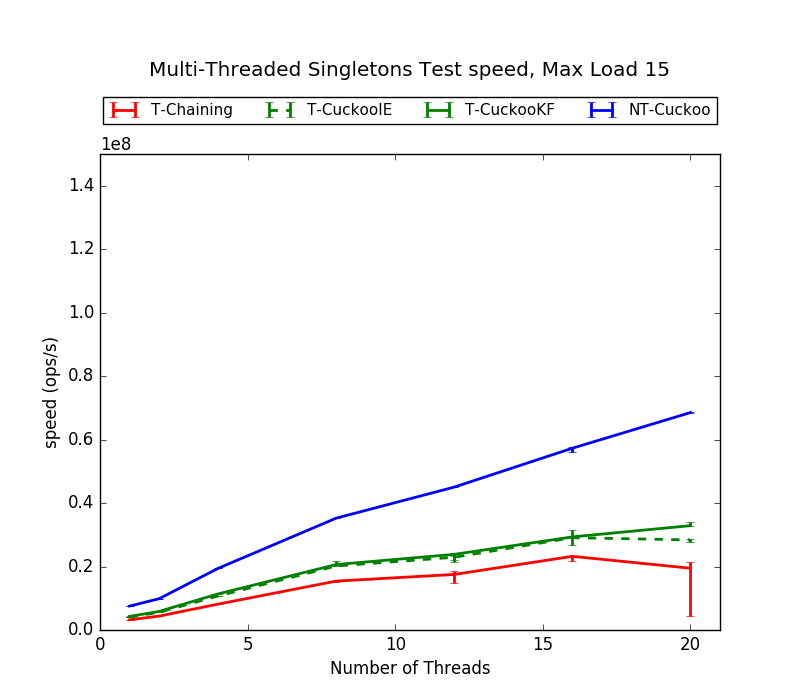
\includegraphics[height=2in]{maps/15HM10K:F34,I33,E33speed.png}
    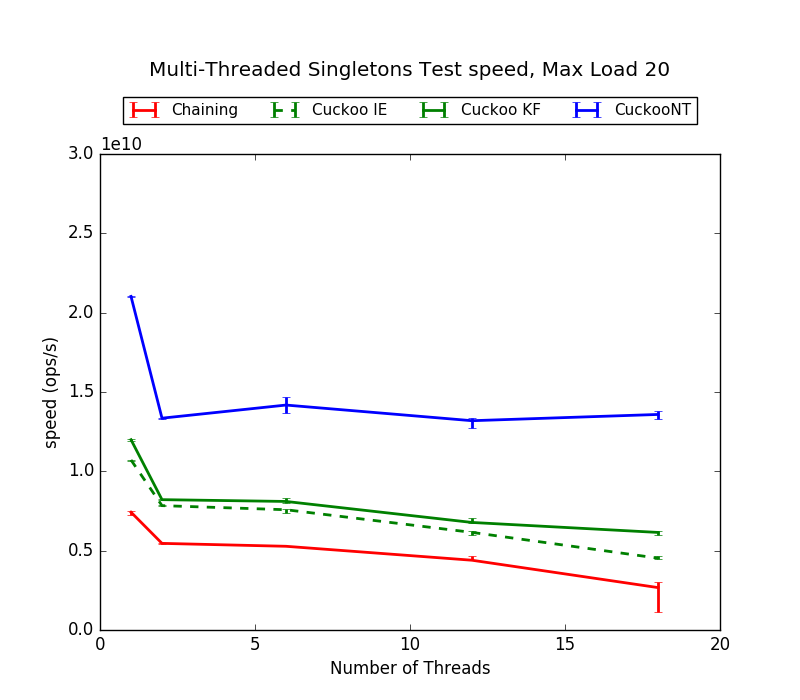
\includegraphics[height=2in]{maps/20HM10K:F34,I33,E33speed.png}
    \\
    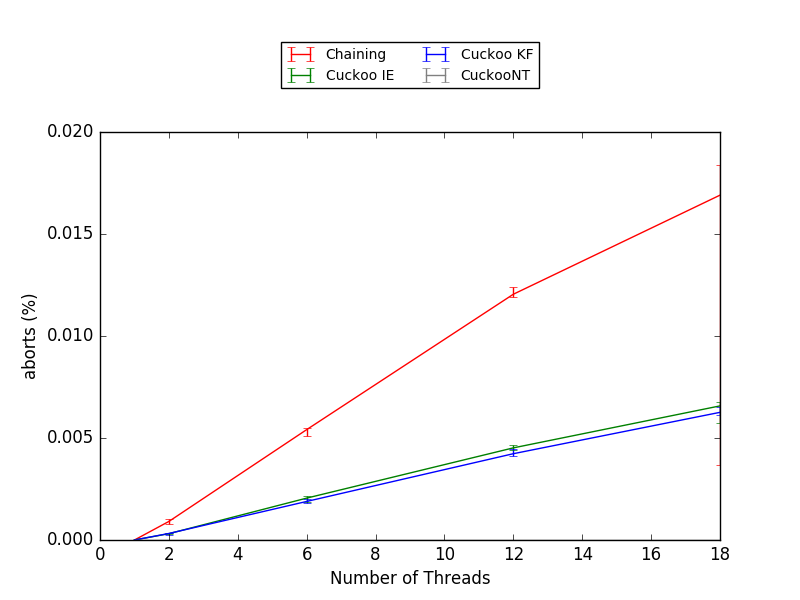
\includegraphics[height=2in]{maps/5HM10K:F34,I33,E33aborts.png}
    $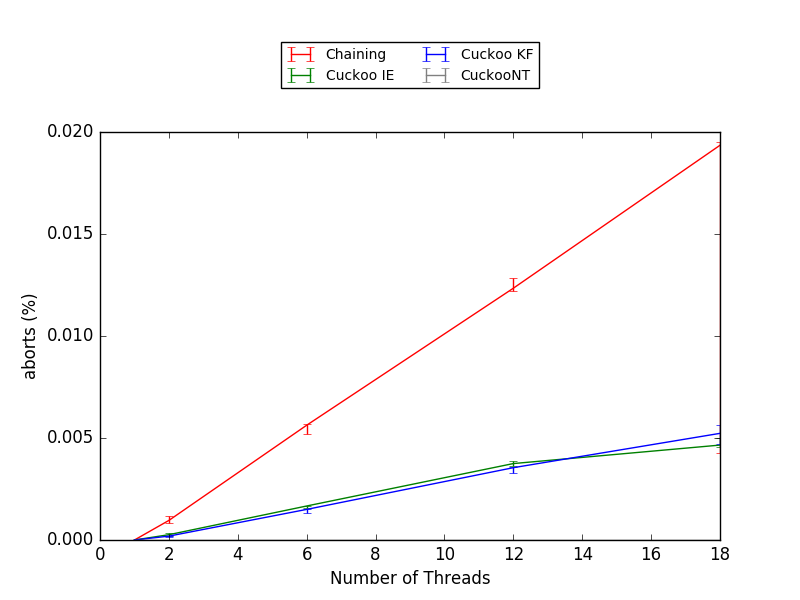
\includegraphics[height=2in]{maps/10HM10K:F34,I33,E33aborts.png}
    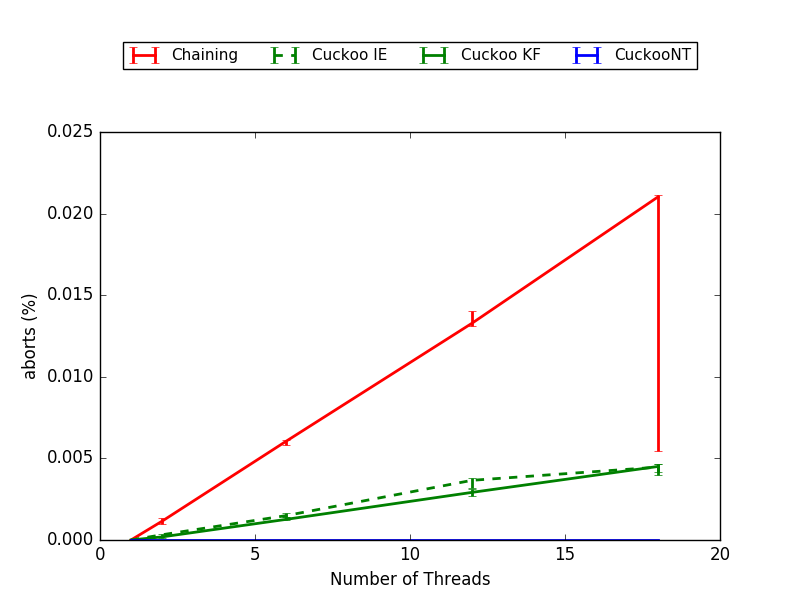
\includegraphics[height=2in]{maps/15HM10K:F34,I33,E33aborts.png}
    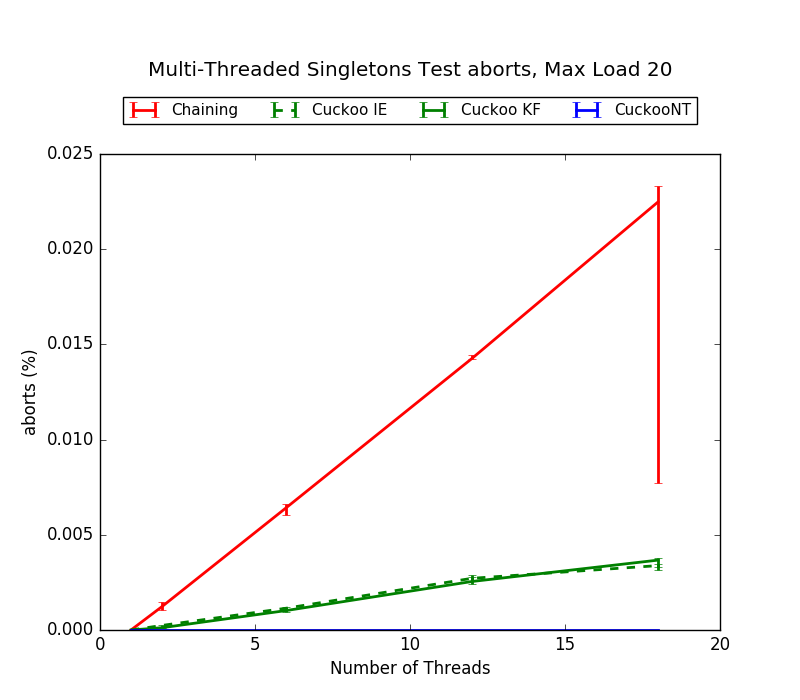
\includegraphics[height=2in]{maps/20HM10K:F34,I33,E33aborts.png}
    \\
    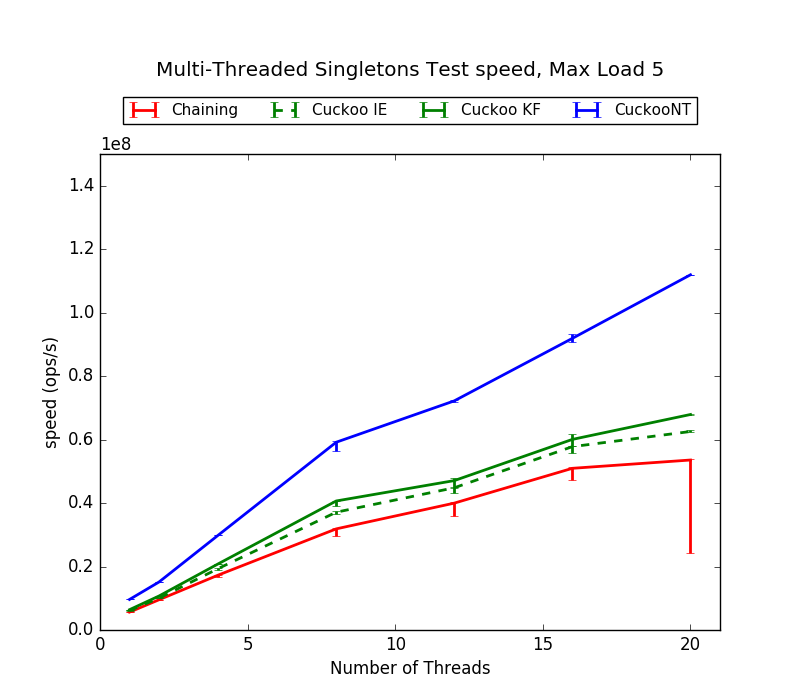
\includegraphics[height=2in]{maps/5HM10K:F90,I5,E5speed.png}
    $\includegraphics[height=2in]{maps/10HM10K:F90,I5,E5speed.png}
    \includegraphics[height=2in]{maps/15HM10K:F90,I5,E5speed.png}
    \includegraphics[height=2in]{maps/20HM10K:F90,I5,E5speed.png}
    \\
    \includegraphics[height=2in]{maps/5HM10K:F90,I5,E5aborts.png}
    $\includegraphics[height=2in]{maps/10HM10K:F90,I5,E5aborts.png}
    \includegraphics[height=2in]{maps/15HM10K:F90,I5,E5aborts.png}
    \includegraphics[height=2in]{maps/20HM10K:F90,I5,E5aborts.png}
\caption{Hashmap with 10K Buckets}
\label{fig:ntqueues}
\end{figure}



\chapter{Future Work and Conclusion}

\section{Future Work}
To further increase performance, our data structures can be specialized for singleton transactions. As we saw in the commutativity discussions of Chapter~\ref{commutativity} and Chapter~\ref{hashmap}, the commutativity between singleton transactions is equivalent to the commutativity between single operations. Special treatment of singleton transactions allows singletons to avoid transactional overhead that is necessary to synchronize multi-operation transactions. However, singletons would need to be carefully handled in the cases in which they interleave with multi-operation transactions. 

We would also like to further test the idea that only those highly-concurrent data structures whose interfaces do not suffer from a high loss of commutativity in a transactional setting will scale well in a transactional setting. Given a concurrent data structure with this property, we hope to construct more transactional STO data structures that perform and scale well.
For concurrent data structures whose performance is crippled in a transactional setting (such as the FIFO queue or priority queue), alternative interfaces for the data structures, such as the one we proposed for the queue, can be explored. These data structure specifications can be tuned to provide some useful guarantees beyond that of a simple concurrent data structure when in a transactional setting while still allowing concurrent algorithms to achieve high performance.

\section{Conclusion}
This thesis argues that retaining the performance benefits and scalability of highly-concurrent data structure algorithms within a transactional framework such as STO is contingent upon the amount of commutativity that is lost when transactions must be supported. The amount of commutativity between transactions determines the amount of independence between the synchronization strategy used by the highly-concurrent algorithm and the transactional bookkeeping and mechanisms that must be added to synchronize transactions.

Our work with the flat combining queues demonstrates that, while there is a large performance gap between our naively-concurrent transactional queues and the best-performing non-transactional, concurrent queue (the flat combining queue), the flat combining queue suffers crippling performance loss when moved into STO. This is because the flat combining technique relies on operation commutativity that is disallowed in a transactional setting, and that the modifications to flat combining required to support transactions reduce the effectiveness of the flat combining technique. Through exploration of an alternative queue specification that allows for greater operation commutativity in a transactional setting, we provide evidence that the effectiveness of the flat combining technique is dependent on operation commutativity.

As an example of the opposite phenomenon, in which a concurrent algorithm retains its performance benefits and scalability, we look to cuckoo and chaining hashing algorithms. This is because both cuckoo and chaining hashmaps experience few added commutativity constraints in a transactional setting.
Furthermore, the beneficial properties of cuckoo hashmaps (such as good performance in a small hashmap with several values in each bucket) are present even in a transactional setting. This is because the cuckoo hashing synchronization algorithm can be implemented independently of the transactional bookkeeping to support transactions: the lack of added commutativity constraints in the transactional setting means that the concurrent cuckoo hashmap algorithm can be made transactional without fundamentally changing its behavior.

Our results provide a way to determine in advance whether a highly-concurrent, non-transactional data structure can be integrated with STO while still achieving high scalability and performance. By evaluating the loss of commutativity in a particular data structure's interface when moving from a non-transactional in a transactional setting, we also evaluate how much impact the modifications necessary to support transactions will have on performance and scalability. This general method allows us to explain why and how different transactional data structures often achieve unexpected performance. We hope to use this method to prevent such surprises in the future.


\singlespacing

\clearpage
\bibliography{thesis}
\addcontentsline{toc}{chapter}{References}
\bibliographystyle{abbrv}
%\chapter*{Colophon}

\begin{center}
\parbox{200pt}{\raggedright\lettrine[lines=3,slope=-2pt,nindent=-4pt]{\textcolor{Crimson}{T}}{his thesis was typeset} using \LaTeX, originally developed by Leslie Lamport and based on Donald Knuth's \TeX. The body text is set in 11 point Arno Pro, designed by Robert Slimbach in the style of book types from the Aldine Press in Venice, and issued by Adobe in 2007. A template, which can be used to format a PhD thesis with this look and feel, has been released under the permissive \textsc{mit} (\textsc{x}11) license, and can be found online at \href{https://github.com/suchow/}{github.com/suchow/} or from the author at \href{mailto:suchow@fas.harvard.edu}{suchow@post.harvard.edu}.
}
\end{center}

\clearpage
\appendix

\appendixpage
\addappheadtotoc

\chapter{Queue Results}
\label{app:queues}

\vspace{-20pt}
\section{Cache Misses}
\begin{figure}[H]
    \centering
    \includegraphics[width=0.66\textwidth]{fcqueues/cm.png}
    \caption{Queue Cache Misses}
    \caption*{
Cache misses are recorded by running the Multi-Thread Singletons Test benchmark with 8 threads, with each thread performing 9M transactions, under the profiling tool Performance Events for Linux (\texttt{perf}). The sampling period is set to 1000, meaning that every 1000th cache miss is recorded.
    In these results, we report the number of cache misses reported by perf (approximately 1/1000 of the actual number of cache misses).}
\label{fig:qcm}
\end{figure}

\section{Performance of Non-transactional Concurrent Queues}
\begin{figure}[H]
    \centering
    \includegraphics[width=0.65\textwidth]{concurrent/allQ:RandSingleOps10000.png}
    \includegraphics[width=0.65\textwidth]{concurrent/allQ:RandSingleOps100000.png}
    \caption{Non-transactional, Concurrent Queues vs. Transactional Queues: Multi-Thread Singletons Test}
\end{figure}
\begin{figure}[H]
    \centering
    \includegraphics[width=\textwidth]{concurrent/allQ:PushPop.png}
    \caption{Non-transactional, Concurrent Queues vs. Transactional Queues: Push-Pop Test}
\end{figure}

\section{Performance of Various Transactional Queues}
\begin{figure}[H]
    \centering
    \includegraphics[width=0.85\textwidth]{fcqueues/allQ:RandSingleOps10000.png}
    \vspace{20pt}
    \includegraphics[width=0.85\textwidth]{fcqueues/allQ:RandSingleOps100000.png}
    \caption{Various Transactional Queues: Multi-Thread Singletons Test}
\end{figure}
\begin{figure}[H]
    \centering
    \includegraphics[width=\textwidth]{fcqueues/allQ:PushPop.png}
    \caption{Various Transactional Queues: Push-Pop Test}
\end{figure}

\section{Abort Rate Results}
\label{app:queue_mt}

\begin{table}[H]
\begin{figure}[H]
    \centering
    \begin{tabular}{|c|c|c|}
\hline
\multirow{2}{*}{Queue} & \multicolumn{2}{c|}{Initial Size}\\\cline{2-3}& \qquad 10000 \qquad\quad & \qquad 100000\qquad\quad\\
\hline
\hline
T-QueueO & 0.00001 & 0.00001\\
T-QueueP & 1.54560 & 1.60886\\
T-FCQueue & 0.62494 & 1.62620\\
WT-FCQueue & 0.00000 & 0.00000\\
\hline\end{tabular}

    \caption*{Push-Pop Test}
\end{figure}
\begin{figure}[H]
    \centering
        \begin{tabular}{|c|c|c|c|}
\hline
\multirow{2}{*}{Queue} & \multicolumn{3}{c|}{\#Threads}\\\cline{2-4}& \quad 4 & 12 & 20\\
\hline
\hline
T-QueueO & 10.21210 & 7.46284 & 6.33827\\
T-QueueP & 2.84958 & 2.26892 & 2.32787\\
NT-FCQueueWrapped & 0.00000 & 0.00000 & 0.00000\\
T-FCQueue & 6.08289 & 4.78435 & 5.33221\\
WT-FCQueue & 0.00000 & 0.00000 & 0.00000\\
\hline\end{tabular}

    \caption*{Multi-Thread Singletons Test: Initial Size 10000}
\end{figure}
\begin{figure}[H]
    \centering
    \begin{tabular}{|c|c|c|c|}
\hline
\multirow{2}{*}{Queue} & \multicolumn{3}{c|}{\#Threads Abort Rate (\%)}\\\cline{2-4}& \quad 4 & 12 & 20\\
\hline
\hline
T-Queue1 & 9.405 & 6.841 & 6.303\\
T-Queue2 & 2.809 & 2.324 & 2.446\\
WT-Queue & 16.600 & 59.998 & 71.140\\
NT-FCQueueWrapped & 0.000 & 0.000 & 0.000\\
T-FCQueue & 4.436 & 3.521 & 4.207\\
WT-FCQueue & 0.000 & 0.000 & 0.000\\
\hline\end{tabular}

    \caption*{Multi-Thread Singletons Test: Initial Size 100000}
\end{figure}
    \caption{Queue Test Abort Rate Results}
\end{table}

\chapter{Hashmap Results}

\section{Cache Misses}

The results are collected by evaluating the Multi-Thread Singletons Test with each thread running 10M transactions under the profiling tool Performance Events for Linux (\texttt{perf}). The sampling period is set to 1000, meaning that every 1000th cache miss is recorded.

In these figures, we report the number of cache misses reported by perf (approximately 1/1000 of the actual number of cache misses.)

    \begin{figure}[H]
    \centering
        {\includegraphics[width=0.5\textwidth]{maps/5cm.png}}
        \caption{Hashmap Cache Misses: Maximum Fullness 5}
    \end{figure}

    \begin{figure}[H]
    \centering
        {\includegraphics[width=0.5\textwidth]{maps/10cm.png}}
        \caption{Hashmap Cache Misses: Maximum Fullness 10}
    \end{figure}

    \begin{figure}[H]
    \centering
        {\includegraphics[width=0.5\textwidth]{maps/15cm.png}}
        \caption{Hashmap Cache Misses: Maximum Fullness 15}
    \end{figure}


\newpage
\section{Multi-Thread Singleton Test Results: 33\% Find, 33\% Insert, 33\% Erase}

\subsection{Maximum Fullness 5}

\begin{figure}[H]
    \centering
    \caption{Hashmap Performance (33F/33I/33E): 10K Buckets, Maximum Fullness 5}
    \includegraphics[width=0.5\textwidth]{maps/5HM10K:F34,I33,E33.png} 
    \begin{tabular}{|c|c|c|c|}
\hline
\multirow{2}{*}{Hashmap} & \multicolumn{3}{c|}{\#Threads}\\\cline{2-4}& 4 & 12 & 20\\
\hline
\hline
T-Chaining & 0.00325 & 0.01291 & 0.01843\\
T-CuckooA & 0.00108 & 0.00487 & 0.00773\\
T-CuckooKF & 0.00100 & 0.00483 & 0.00799\\
NT-Cuckoo & 0.00000 & 0.00000 & 0.00000\\
\hline
\end{tabular}

\end{figure}

\begin{figure}[H]
    \centering
    \caption{Hashmap Performance (33F/33I/33E): 125K Buckets, Maximum Fullness 5}
    \includegraphics[width=0.5\textwidth]{maps/10HM125K:F34,I33,E33.png} 
    \begin{tabular}{|c|c|c|c|}
\hline
\multirow{2}{*}{Hashmap} & \multicolumn{3}{c|}{\#Threads Abort Rate (\%)}\\\cline{2-4}& 4 & 12 & 20\\
\hline
\hline
T-Chaining & 0.000 & 0.001 & 0.002\\
T-CuckooIE & 0.000 & 0.001 & 0.001\\
T-CuckooKF & 0.000 & 0.000 & 0.001\\
NT-Cuckoo & 0.000 & 0.000 & 0.000\\
\hline
\end{tabular}

\end{figure}

\begin{figure}[H]
    \centering
    \caption{Hashmap Performance (33F/33I/33E): 1M Buckets, Maximum Fullness 5}
    \includegraphics[width=0.5\textwidth]{maps/15HM1M:F34,I33,E33.png} 
    \begin{tabular}{|c|c|c|c|c|c|c|}
\hline
\multirow{2}{*}{Hashmap} & \multicolumn{6}{c|}{\#Threads}\\\cline{2-7}& 2 & 4 & 8 & 12 & 16 & 20\\
\hline
\hline
T-Chaining & 0.00002 & 0.00004 & 0.00009 & 0.00012 & 0.00018 & 0.00022\\
T-CuckooA & 0.00000 & 0.00001 & 0.00003 & 0.00004 & 0.00007 & 0.00010\\
T-CuckooKF & 0.00000 & 0.00001 & 0.00002 & 0.00004 & 0.00006 & 0.00009\\
NT-Cuckoo & 0.00000 & 0.00000 & 0.00000 & 0.00000 & 0.00000 & 0.00000\\
\hline
\end{tabular}

\end{figure}

\subsection{Maximum Fullness 10}

\begin{figure}[H]
    \centering
    \caption{Hashmap Performance (33F/33I/33E): 10K Buckets, Maximum Fullness 10}
    \includegraphics[width=0.5\textwidth]{maps/10HM10K:F34,I33,E33.png} 
    \begin{tabular}{|c|c|c|c|}
\hline
\multirow{2}{*}{Hashmap} & \multicolumn{3}{c|}{\#Threads Abort Rate (\%)}\\\cline{2-4}& 4 & 12 & 20\\
\hline
\hline
T-Chaining & 0.003 & 0.013 & 0.021\\
T-CuckooIE & 0.001 & 0.004 & 0.005\\
T-CuckooKF & 0.001 & 0.004 & 0.007\\
NT-Cuckoo & 0.000 & 0.000 & 0.000\\
\hline
\end{tabular}

\end{figure}

\begin{figure}[H]
    \centering
    \caption{Hashmap Performance (33F/33I/33E): 125K Buckets, Maximum Fullness 10}
    \includegraphics[width=0.5\textwidth]{maps/10HM125K:F34,I33,E33.png} 
    \begin{tabular}{|c|c|c|c|}
\hline
\multirow{2}{*}{Hashmap} & \multicolumn{3}{c|}{\#Threads}\\\cline{2-4}& 4 & 12 & 20\\
\hline
\hline
T-Chaining & 0.000 & 0.002 & 0.002\\
T-CuckooIE & 0.000 & 0.000 & 0.001\\
T-CuckooKF & 0.000 & 0.000 & 0.001\\
NT-Cuckoo & 0.000 & 0.000 & 0.000\\
\hline
\end{tabular}

\end{figure}

\begin{figure}[H]
    \centering
    \caption{Hashmap Performance (33F/33I/33E): 1M Buckets, Maximum Fullness 10}
    \includegraphics[width=0.5\textwidth]{maps/10HM1M:F34,I33,E33.png} 
    \begin{tabular}{|c|c|c|c|}
\hline
\multirow{2}{*}{Hashmap} & \multicolumn{3}{c|}{\#Threads}\\\cline{2-4}& 4 & 12 & 20\\
\hline
\hline
T-Chaining & 0.00004 & 0.34599 & 0.13496\\
T-CuckooA & 0.00001 & 0.15493 & 0.04467\\
T-CuckooKF & 0.00001 & 0.09270 & 0.06208\\
NT-Cuckoo & 0.00000 & 0.00000 & 0.00000\\
\hline
\end{tabular}

\end{figure}

\subsection{Maximum Fullness 15}

\begin{figure}[H]
    \centering
    \caption{Hashmap Performance (33F/33I/33E): 10K Buckets, Maximum Fullness 15}
    \includegraphics[width=0.5\textwidth]{maps/15HM10K:F34,I33,E33.png} 
    \begin{tabular}{|c|c|c|c|}
\hline
\multirow{2}{*}{Hashmap} & \multicolumn{3}{c|}{\#Threads}\\\cline{2-4}& 4 & 12 & 20\\
\hline
\hline
T-Chaining & 0.004 & 0.015 & 0.023\\
T-CuckooIE & 0.001 & 0.004 & 0.005\\
T-CuckooKF & 0.001 & 0.003 & 0.005\\
NT-Cuckoo & 0.000 & 0.000 & 0.000\\
\hline
\end{tabular}

\end{figure}

\begin{figure}[H]
    \centering
    \caption{Hashmap Performance (33F/33I/33E): 125K Buckets, Maximum Fullness 15}
    \includegraphics[width=0.5\textwidth]{maps/15HM125K:F34,I33,E33.png} 
    \begin{tabular}{|c|c|c|c|}
\hline
\multirow{2}{*}{Hashmap} & \multicolumn{3}{c|}{\#Threads Abort Rate (\%)}\\\cline{2-4}& 4 & 12 & 20\\
\hline
\hline
T-Chaining & 0.000 & 0.002 & 0.003\\
T-CuckooIE & 0.000 & 0.001 & 0.001\\
T-CuckooKF & 0.000 & 0.000 & 0.001\\
NT-Cuckoo & 0.000 & 0.000 & 0.000\\
\hline
\end{tabular}

\end{figure}

\begin{figure}[H]
    \centering
    \caption{Hashmap Performance (33F/33I/33E): 1M Buckets, Maximum Fullness 15}
    \includegraphics[width=0.5\textwidth]{maps/15HM1M:F34,I33,E33.png} 
    \begin{tabular}{|c|c|c|c|c|c|c|}
\hline
\multirow{2}{*}{Hashmap} & \multicolumn{6}{c|}{\#Threads}\\\cline{2-7}& 2 & 4 & 8 & 12 & 16 & 20\\
\hline
\hline
T-Chaining & 0.00002 & 0.00005 & 0.14779 & 0.08940 & 0.00022 & 0.00027\\
T-CuckooA & 0.00000 & 0.00001 & 0.03164 & 0.01825 & 0.00005 & 0.00008\\
T-CuckooKF & 0.00000 & 0.00001 & 0.01399 & 0.00735 & 0.00005 & 0.00007\\
NT-Cuckoo & 0.00000 & 0.00000 & 0.00000 & 0.00000 & 0.00000 & 0.00000\\
\hline
\end{tabular}

\end{figure}

\newpage
\section{Multi-Thread Singleton Test Results: 90\% Find, 5\% Insert, 5\% Erase}

\subsection{Maximum Fullness 5}

\begin{figure}[H]
    \centering
    \caption{Hashmap Performance (34F/5I/5E): 10K Buckets, Maximum Fullness 5}
    \includegraphics[width=0.5\textwidth]{maps/5HM10K:F90,I5,E5.png} 
    \begin{tabular}{|c|c|c|c|}
\hline
\multirow{2}{*}{Hashmap} & \multicolumn{3}{c|}{\#Threads}\\\cline{2-4}& 4 & 12 & 20\\
\hline
\hline
T-Chaining & 0.001 & 0.003 & 0.005\\
T-CuckooIE & 0.001 & 0.001 & 0.002\\
T-CuckooKF & 0.000 & 0.001 & 0.002\\
NT-Cuckoo & 0.000 & 0.000 & 0.000\\
\hline
\end{tabular}

\end{figure}

\begin{figure}[H]
    \centering
    \caption{Hashmap Performance (34F/5I/5E): 125K Buckets, Maximum Fullness 5}
    \includegraphics[width=0.5\textwidth]{maps/10HM125K:F90,I5,E5.png} 
    \begin{tabular}{|c|c|c|c|}
\hline
\multirow{2}{*}{Hashmap} & \multicolumn{3}{c|}{\#Threads}\\\cline{2-4}& 4 & 12 & 20\\
\hline
\hline
T-Chaining & 0.00006 & 0.00023 & 0.00038\\
T-CuckooA & 0.00003 & 0.00011 & 0.00026\\
T-CuckooKF & 0.00003 & 0.00011 & 0.00026\\
NT-Cuckoo & 0.00000 & 0.00000 & 0.00000\\
\hline
\end{tabular}

\end{figure}

\begin{figure}[H]
    \centering
    \caption{Hashmap Performance (34F/5I/5E): 1M Buckets, Maximum Fullness 5}
    \includegraphics[width=0.5\textwidth]{maps/15HM1M:F90,I5,E5.png} 
    \begin{tabular}{|c|c|c|c|}
\hline
\multirow{2}{*}{Hashmap} & \multicolumn{3}{c|}{\#Threads}\\\cline{2-4}& 4 & 12 & 20\\
\hline
\hline
T-Chaining & 0.00001 & 0.00003 & 0.00006\\
T-CuckooA & 0.00001 & 0.00001 & 0.00003\\
T-CuckooKF & 0.00000 & 0.00001 & 0.00003\\
NT-Cuckoo & 0.00000 & 0.00000 & 0.00000\\
\hline
\end{tabular}

\end{figure}

\subsection{Maximum Fullness 10}

\begin{figure}[H]
    \centering
    \caption{Hashmap Performance (90F/5I/5E): 10K Buckets, Maximum Fullness 10}
    \includegraphics[width=0.5\textwidth]{maps/10HM10K:F90,I5,E5.png} 
    \begin{tabular}{|c|c|c|c|c|c|c|}
\hline
\multirow{2}{*}{Hashmap} & \multicolumn{6}{c|}{\#Threads}\\\cline{2-7}& 2 & 4 & 8 & 12 & 16 & 20\\
\hline
\hline
T-Chaining & 0.00050 & 0.00100 & 0.00229 & 0.00318 & 0.00409 & 0.00534\\
T-CuckooA & 0.00020 & 0.00057 & 0.00106 & 0.00150 & 0.00178 & 0.00233\\
T-CuckooKF & 0.00020 & 0.00057 & 0.00095 & 0.00140 & 0.00171 & 0.00243\\
NT-Cuckoo & 0.00000 & 0.00000 & 0.00000 & 0.00000 & 0.00000 & 0.00000\\
\hline
\end{tabular}

\end{figure}

\begin{figure}[H]
    \centering
    \caption{Hashmap Performance (90F/5I/5E): 125K Buckets, Maximum Fullness 10}
    \includegraphics[width=0.5\textwidth]{maps/10HM125K:F90,I5,E5.png} 
    \begin{tabular}{|c|c|c|c|c|c|c|}
\hline
\multirow{2}{*}{Hashmap} & \multicolumn{6}{c|}{Number of Threads Abort Rate (\%)}\\\cline{2-7}& 2 & 4 & 8 & 12 & 16 & 20\\
\hline
\hline
T-Chaining & 0.000 & 0.000 & 0.000 & 0.000 & 0.001 & 0.001\\
T-CuckooIE & 0.000 & 0.000 & 0.000 & 0.000 & 0.000 & 0.001\\
T-CuckooKF & 0.000 & 0.000 & 0.000 & 0.000 & 0.000 & 0.001\\
NT-Cuckoo & 0.000 & 0.000 & 0.000 & 0.000 & 0.000 & 0.000\\
\hline
\end{tabular}

\end{figure}

\begin{figure}[H]
    \centering
    \caption{Hashmap Performance (90F/5I/5E): 1M Buckets, Maximum Fullness 10}
    \includegraphics[width=0.5\textwidth]{maps/10HM1M:F90,I5,E5.png} 
    \begin{tabular}{|c|c|c|c|}
\hline
\multirow{2}{*}{Hashmap} & \multicolumn{3}{c|}{\#Threads}\\\cline{2-4}& 4 & 12 & 20\\
\hline
\hline
T-Chaining & 0.00001 & 0.00034 & 0.00022\\
T-CuckooA & 0.00000 & 0.00050 & 0.00007\\
T-CuckooKF & 0.00000 & 0.00026 & 0.00003\\
NT-Cuckoo & 0.00000 & 0.00000 & 0.00000\\
\hline
\end{tabular}

\end{figure}

\subsection{Maximum Fullness 15}

\begin{figure}[H]
    \centering
    \caption{Hashmap Performance (90F/5I/5E): 10K Buckets, Maximum Fullness 15}
    \includegraphics[width=0.5\textwidth]{maps/15HM10K:F90,I5,E5.png} 
    \begin{tabular}{|c|c|c|c|c|c|c|}
\hline
\multirow{2}{*}{Hashmap} & \multicolumn{6}{c|}{\#Threads}\\\cline{2-7}& 2 & 4 & 8 & 12 & 16 & 20\\
\hline
\hline
T-Chaining & 0.00030 & 0.00103 & 0.00266 & 0.00378 & 0.00449 & 0.00584\\
T-CuckooA & 0.00025 & 0.00065 & 0.00115 & 0.00166 & 0.00205 & 0.00250\\
T-CuckooKF & 0.00010 & 0.00068 & 0.00111 & 0.00163 & 0.00196 & 0.00262\\
NT-Cuckoo & 0.00000 & 0.00000 & 0.00000 & 0.00000 & 0.00000 & 0.00000\\
\hline
\end{tabular}

\end{figure}

\begin{figure}[H]
    \centering
    \caption{Hashmap Performance (90F/5I/5E): 125K Buckets, Maximum Fullness 15}
    \includegraphics[width=0.5\textwidth]{maps/15HM125K:F90,I5,E5.png} 
    \begin{tabular}{|c|c|c|c|}
\hline
\multirow{2}{*}{Hashmap} & \multicolumn{3}{c|}{\#Threads}\\\cline{2-4}& 4 & 12 & 20\\
\hline
\hline
T-Chaining & 0.00009 & 0.00027 & 0.00047\\
T-CuckooA & 0.00004 & 0.00013 & 0.00023\\
T-CuckooKF & 0.00002 & 0.00007 & 0.00018\\
NT-Cuckoo & 0.00000 & 0.00000 & 0.00000\\
\hline
\end{tabular}

\end{figure}

\begin{figure}[H]
    \centering
    \caption{Hashmap Performance (90F/5I/5E): 1M Buckets, Maximum Fullness 15}
    \includegraphics[width=0.5\textwidth]{maps/15HM1M:F90,I5,E5.png} 
    \begin{tabular}{|c|c|c|c|}
\hline
\multirow{2}{*}{Hashmap} & \multicolumn{3}{c|}{\#Threads}\\\cline{2-4}& 4 & 12 & 20\\
\hline
\hline
T-Chaining & 0.00001 & 0.00636 & 0.00016\\
T-CuckooA & 0.00000 & 0.00001 & 0.00037\\
T-CuckooKF & 0.00000 & 0.00001 & 0.00006\\
NT-Cuckoo & 0.00000 & 0.00000 & 0.00000\\
\hline
\end{tabular}

\end{figure}

\iffalse
\begin{table}[H]
    \centering
\begin{tabular}{|c|c|c|c|c|c|}
    find(x)-find(x) & insert(x)-insert(x) & erase(x)-erase(x) & find(x)-insert(x) & find(x)-erase(x) & insert(x)-erase(x)\\
    \hline
    & W-W, W-R & W-W, W-R & R-W & R-W & W-W, W-R
\end{tabular}
    \caption*{R-R relations are not shown.}
    \caption{Dependencies of pairs of hashmap operations}
    \label{table:hashmapsimpledeps}
\end{table}
\fi



\end{document}
